\section{C Implementation and Infrastructure}
\label{sec:cport}

The fixed-point reference model of Section~\ref{sec:fixed} answers
\emph{whether} integer arithmetic preserves the link performance; the C
port (\texttt{cport/}) answers whether the system \emph{fits} a DSP or
microcontroller.  It is portable C99 with no \texttt{malloc} and no
floating point on the signal path (doubles remain on the control plane
--- dB values and timers --- as in the model), and covers the entire
feature family: both FEC families, all three modulations and link
modes, the gated two-stage frequency search, HARQ combining, calibrated
LLRs, the integer SNR estimator, the full link layer, and a streaming
receiver architecture for MCU deployment.

\subsection{Bit-Exact Porting Methodology}
\label{sec:cport_method}

Every module is validated against \emph{golden vectors} generated from
the Python fixed-point model (\texttt{gen\_vectors.py}): inputs and
expected outputs are dumped as C headers and compared with
\texttt{memcmp} --- no tolerances anywhere.  Whole transmit frames
(up to 260\,k samples for EXTREME) are compared through 64-bit
FNV-1a hashes over every \texttt{int16} sample, with the first 64
samples embedded verbatim for debuggability.  Two rules keep the
comparison honest:

\begin{itemize}
    \item \textbf{ROMs are dumped, never recomputed.}  Twiddles,
          preamble blocks, pilot symbols, LDPC graph, ladder tables and
          detection kernels all come from the Python model; a C-side
          reimplementation of table generation would risk silently
          diverging in rounding.
    \item \textbf{Width findings are documented, not patched over.}
          Every intermediate that exceeds a naive width estimate
          (Viterbi path metrics, BFP energy sums, the ZC metric's
          Q-scaling) is recorded in \texttt{WIDTHS.md} with its measured
          range, so an RTL implementation inherits the analysis.
\end{itemize}

The suite currently runs \textbf{79 checks} across six binaries
(primitives, bit pipeline, TX frames, RX demodulation, streaming
receiver, link layer).  RX genie vectors are self-hosting: clean frames
are rebuilt by the bit-exact C transmitter inside the test, so only the
Python detection genie (start sample, CFO word) and expected bits are
dumped.

\subsection{Streaming Receiver}
\label{sec:cport_stream}

The frame-at-once reference receiver is impractical on an MCU (it wants
the whole capture in memory), so \texttt{rx\_stream.c} implements a
ring-buffer state machine (\textsc{search} $\rightarrow$ \textsc{zc}
$\rightarrow$ \textsc{header} $\rightarrow$ \textsc{data}) fed in
arbitrary chunks.  The tone-detection stage is necessarily causal and
diverges from the model in two documented ways: block exponents and the
noise floor are windowed (a streaming receiver cannot know the whole
capture's minimum exponent, and the model's whole-capture \emph{median}
floor is acausal), and detection commits on a local metric peak ---
when the above-threshold region ends or the argmax stays stable for a
full window span --- instead of a global argmax.  On the golden corpus
the streaming receiver lands on the identical tone anchor for clean
frames, making everything downstream bit-identical to the
frame-at-once path.

Memory is dominated by sample history, and two measurements shaped the
final architecture:

\begin{itemize}
    \item \textbf{The ring only needs to cover the Zadoff--Chu
          re-anchor lookback, not the preamble.}  The tone stage is
          incremental (each 512-sample block folds into a
          $\approx$540-byte summary; raw tone samples are never
          re-read).  A permanent high-water-mark diagnostic
          (\texttt{rxs\_ring\_hwm}) measured the deepest lookback over
          the corpus at 8\,510 / 32\,318 / 124\,478 samples per mode.
    \item \textbf{One shared raw ring serves every instance.}  All
          mode-instances listen to the same audio (the preamble root
          self-labels the mode), so concurrent instances write
          identical samples and a single \texttt{int16} ring of
          147\,456 samples (288\,KB) replaces per-instance analytic
          rings.  The analytic signal is reconstructed on extraction
          (Hilbert-on-read), bit-identical to the former write-time
          FIR --- and measured \emph{faster}, because the 63-tap filter
          now runs only on consumed regions rather than on every
          sample in every instance.
\end{itemize}

\subsection{Protocol Extensions}
\label{sec:cport_proto}

Three extensions beyond the Python reference address the fixed
per-frame overhead (preamble + header $\approx$0.64\,s in NORMAL mode)
that dominates air time at the top rungs:

\begin{itemize}
    \item \textbf{Selective-repeat burst ARQ.}  Bulk transfers send up
          to a window of frames back-to-back, answered by one bitmap
          acknowledgment (NACK-by-omission).  The two flag combinations
          impossible in the legacy protocol serve as burst frame types,
          so the legacy path is untouched.
    \item \textbf{Extended frames.}  The article's header \texttt{len}
          field counts packet \emph{bits} (255 max
          $\rightarrow$ 27-byte payloads).  An unused header type
          codepoint reinterprets \texttt{len} as payload \emph{bytes},
          allowing 255-byte payloads (2\,076-bit packets) behind a
          single preamble.  Burst fragment size scales with the
          engage-time rung (200\,B at rung $\ge$10, 100\,B at $\ge$7,
          else 25\,B).
    \item \textbf{Streamed burst windows.}  A whole selective-repeat
          window is transmitted behind one preamble and header
          (Sections~\ref{sec:stream} and~\ref{sec:burstwin}) instead
          of one preamble per fragment.  \texttt{tx\_build\_burst}
          waveforms are bit-exact against the fixed-point model, and
          both receivers can follow a burst: the frame-at-once path
          re-runs the recording through \texttt{rxd\_receive\_burst}
          and re-locks on each Zadoff--Chu block, while the streaming
          receiver steps to the next block at its deterministic offset
          via \texttt{rxs\_continue\_burst}.
\end{itemize}

A streamed burst carries only full-size fragments; the short tail of a
transfer always travels as its own frame, because the receiver derives
the message length from that final fragment's own length.  The
acknowledgment request rides on the burst's \emph{first} block as well
as its last, so a peer that cannot follow the stream still answers and
the sender learns by bitmap rather than by waiting out a timeout.

That receive-side continuation is also where the sharpest bug of this
work appeared.  While the streaming receiver is stepping through
blocks it is not running the preamble detector, so a continuation that
does not know where to stop makes the receiver deaf for one block-time
per phantom block.  An early version re-armed its block counter on
every successful block and therefore never learned that a burst had
ended: it chased up to seven blocks that were never sent,
$\approx$12\,s of deafness landing squarely on the peer's next burst,
which timed out and retried indefinitely.  The transmitter marks the
last block of a burst with the acknowledgment request, which is the
stop signal --- qualified as ``set \emph{and} not the first block of
this stream'', since the first carries it too.

Measured on the virtual channel: a 250-byte transfer completes in
3 frames instead of $\approx$20 for stop-and-wait, and a 5\,000-byte
file drops from 211 transmitted frames (legacy) to 45, holding the top
QAM16 rung throughout.  Streaming the window compounds this: a
250-byte transfer at 25-byte fragments takes 4 transmissions streamed
against 13 after falling back to per-frame bursts, and a 14\,kB file
over a $+20$\,dB channel takes 76 transmissions streamed against 187
per-frame.

A fourth extension sits above the protocol rather than inside it.
Nothing in the chain compressed, while every comparable HF system does
--- Winlink's B2F, VARA, and PACTOR all compress before transmitting.
Files are now DEFLATEd whole and the compressed stream is what gets
split into parts; compressing each part separately would discard most
of the ratio, since the dictionary never warms up.  A distinct envelope
magic marks the compressed form, so a peer that predates it sees an
unknown message rather than misparsing a structurally valid one, and
the transmitter falls back to sending raw whenever compression fails to
shrink the payload.  Compression lives at the application layer
precisely so the C port stays dependency-free: an embedded build
substitutes miniz or heatshrink, with plain DEFLATE on the wire either
way.  Measured on a 14\,kB configuration file: 14\,162 bytes to
5\,015 on air, $2.82\times$.  The honest qualification is that
transmissions fell only $1.4\times$ and wall-clock delivery
$1.6\times$, because acknowledgments and the rate-ladder bootstrap do
not compress --- the ratio applies to the part of an exchange that is
payload, not to the exchange.  Supporting endpoints added alongside: a
diagnostic event stream (every TX/RX, timeout, rung change annotated
with the controller inputs that caused it, burst state transitions)
plus a controller-decision snapshot --- which immediately located a
real bug (burst acknowledgment windows systematically timing out and
poisoning the rate controller toward its hard rung-0 fallback; fixed by
forgiving a window's first miss and budgeting the reply air time for
the actual bitmap at a conservative rung) --- and an external
oscillator fine-tune endpoint (VCTCXO DAC / CAT clarifier actuator
driven by the AFC netting loop, with budget clamping, an anchor role,
and a manual override).

\subsection{Memory and Flash Engineering}
\label{sec:cport_memory}

Table~\ref{tab:cport_flash} shows the measured flash footprint
(\texttt{arm-none-eabi-gcc -mcpu=cortex-m7 -O2}, const tables count
into \texttt{.text}).  Three reductions brought the total from an
initial 242\,KB to $\approx$57\,KB with zero runtime cost and
bit-exactness enforced by the golden tests:

\begin{itemize}
    \item \textbf{Preambles stored as their unique periodic blocks}
          (183\,KB $\rightarrow$ 1.3\,KB): each mode's preamble is
          exactly a 32-sample tone block tiled $2T{\times}4$ times, a
          64-sample tone block tiled $T{\times}2$ times, and one
          128-sample ZC tile (whose tail doubles as the cyclic prefix)
          repeated \texttt{sym\_tile} times --- 224 unique samples per
          mode, re-expanded by modulo indexing.
    \item \textbf{Single-table trigonometry} (18.2\,KB $\rightarrow$
          8\,KB): the NCO sine table and all six FFT twiddle arrays are
          exact index-arithmetic views of one 4096-entry cosine table
          ($\sin[i]=\cos[(i+3N/4) \bmod N]$; twiddles at stride
          $N/n$); the generator asserts the identities at dump time.
    \item \textbf{Packed Viterbi traceback} (1 bit per state per step
          instead of a predecessor byte --- the predecessor is
          $(s{\gg}1) + (\mathrm{bit}{\ll}5)$), and \texttt{int32}
          depuncture buffers: extended-frame Viterbi state fell from
          181\,KB to 42\,KB, bit-identically.
\end{itemize}

\begin{table}[H]
    \centering
    \caption{Measured Cortex-M7 flash footprint (all three modes).}
    \label{tab:cport_flash}
    \small
    \begin{tabular}{@{}lrl@{}}
    \toprule
    \textbf{Object} & \textbf{Flash} & \textbf{Dominant tables} \\
    \midrule
    \texttt{fft.o}        & 9.4\,KB  & 8\,KB shared cosine ROM \\
    \texttt{rx\_detect.o} & 10.5\,KB & ZC kernels + detection masks \\
    \texttt{rx\_stream.o} + \texttt{rx\_demod.o} & 16.9\,KB &
                            frequency-search tables \\
    \texttt{ldpc.o}       & 7.2\,KB  & code graph \\
    \texttt{link.o} + \texttt{station.o} & 7.2\,KB & rate-ladder ROM \\
    \texttt{tx.o}         & 3.5\,KB  & 1.3\,KB preamble blocks \\
    \texttt{dsp.o} + \texttt{conv.o} + others & 3.0\,KB & --- \\
    \midrule
    \textbf{Total}        & \textbf{$\approx$57\,KB} & \\
    \bottomrule
    \end{tabular}
\end{table}

\subsubsection{RAM: Making the Cost Follow the Signal, Not the Capture}

The host reference buffers whole captures because a workstation can
afford to: the transmitter assembled a complete frame before clipping
it, the detector materialised its entire search window, and the
demodulator held a whole recording. Linked for Cortex-M7 that came to
roughly 10\,MB of \texttt{.bss}, which is not an optimisation problem so
much as a statement that the reference had never been asked the
question. Five changes took it to 699\,KB, each verified bit-exact
against the golden vectors on both x86 and Cortex-M7.

\textbf{The transmitter generates on demand} (4.3\,MB $\rightarrow$
10\,kB). The waveform is nothing but short periodic blocks repeated:
tone field A is a 32-sample block, tone B is 64, ZC is 128, and a data
symbol is one 128-sample IFFT tile repeated \texttt{sym\_tile} times
behind a CP that is its own tail. So a generator needs one tile, not one
frame. The obstacle is that the clip threshold is a \emph{whole}-waveform
RMS --- the invariant that makes a burst not the concatenation of
separately built frames. Rather than buffer for it, the generator runs
twice: once to accumulate energy, once to emit. It is a pure function of
its inputs, so the second pass reproduces the first exactly.

\textbf{Detection pulls instead of being handed a window} (2.4\,MB
$\rightarrow$ 220\,kB). The ZC scan sweeps up to 70\,688 samples at
EXTREME --- 5.9\,s of audio --- but its \emph{live} span is only
$\mathrm{preamble\_len}+1$: at position $p$ the correlation reads
$[p, p{+}\mathrm{klen})$ and the energy term reads
$m = p-(ng{-}1)\mathrm{klen}$ and $m+\mathrm{preamble\_len}$, which is
the same leading edge because $ng \cdot \mathrm{klen} =
\mathrm{preamble\_len}$ exactly. Likewise the two lag correlations use
lags of 128 and 64 --- not a fraction of the segment --- so they need a
128-sample delay line however long the segment is. A fetch-by-index
source lets the scan read from the raw \texttt{int16} ring that already
holds the audio, derotating on the way out (the phase at index $k$ is
$k \cdot cw \bmod 2^{32}$, which is what makes random access possible).

\textbf{One arena for scratch that is never co-resident} (646\,kB
$\rightarrow$ 129\,kB). Classifying buffers by \emph{lifetime} rather
than by name: the raw ring, the block summaries and the per-symbol LLR
accumulators carry state across calls and cannot be shared, but
everything else is call-scoped, and the phases are strictly sequential
--- detection finishes before the first symbol is demodulated, demod
before decode. One arena sized by the \emph{largest} phase replaces
their sum. The subtlety worth recording is that demod is the largest,
not detection: \texttt{eval\_hyp}'s derotation scratch is live
\emph{while} the symbol samples still are, because it runs inside the
symbol demodulator. Sizing from the buffer list rather than the actual
nesting would have produced silent corruption.

\textbf{Narrowing the sample and soft-decision types.} Measured peaks
across the whole suite justify each: analytic samples 43\,077 (17 bits
$\rightarrow$ \texttt{int32}), LLRs 1\,211\,062 (21 bits), correlation
magnitudes 780\,982 (20 bits). Products of two narrowed values are
widened explicitly --- on Cortex-M7 that is \texttt{SMULL}/\texttt{SMLAL},
the same instruction count as \texttt{MUL}/\texttt{MLA}, so exactness is
free.

\textbf{Per-instance tone summaries} (204\,kB $\rightarrow$ 94\,kB).
Every receiver instance had been given EXTREME's 128-block ring, but an
instance only ever scans its own mode's window: 15/30/120 blocks.

\begin{table}[H]
    \centering
    \caption{Measured Cortex-M7 RAM (\texttt{-Os}, \texttt{--gc-sections},
             linked image referencing only the streaming APIs).}
    \label{tab:cport_ram}
    \small
    \begin{tabular}{@{}lrl@{}}
    \toprule
    \textbf{Component} & \textbf{RAM} & \textbf{Sized by} \\
    \midrule
    Shared raw \texttt{int16} ring & 160\,KB & EXTREME re-anchor
                                               lookback (67\,134) \\
    Scratch arena (RX 3 phases $+$ TX) & 128.5\,KB & EXTREME ZC
                                                     geometry \\
    Tone summaries, 3 instances & 94\,KB & each instance's own mode \\
    LLR buffers (\texttt{int32}) & 24\,KB & 192\,KB with EXT frames \\
    Message store (pooled) & 3\,KB & 12 slots, peak 6 measured \\
    Everything else & 152\,KB & --- \\
    \midrule
    \textbf{Total, three modes} & \textbf{561\,KB} & 793\,KB with EXT
                                                     frames \\
    Transmit-only image & 27\,KB & \\
    \bottomrule
    \end{tabular}
\end{table}

\textbf{Target fit, corrected.} An earlier estimate put the three-mode
station at $\approx$453\,KB and concluded it fitted the STM32H723xG
($\approx$496\,KB usable data RAM) with margin. The linked image does
not: 699\,KB without extended frames, 929\,KB with. The estimate had
costed per-mode summaries while the code gave every instance the
EXTREME count, and assumed a build without EXT frames. Both were
addressed; three further reductions followed, described below and in
Section~\ref{sec:cport_ontarget}, bringing the figure to 561\,KB. The
conclusion is unchanged in kind --- an H743-class device, not the
H723xG --- but the margin is now comfortable rather than absent.

Nor is a single-mode build the way out, though the arithmetic is
tempting. Rung~0 of the ladder is EXTREME, and rung~0 is where both
stations bootstrap, where the controller drops after four consecutive
losses, and where staleness decay lands; rungs 1--3 are ROBUST. A build
without EXTREME cannot acquire a link at all, nor recover one after a
fade --- which is exactly when 64$\times$ tiling earns its cost.
Per-mode sizing is a capability decision, not a memory knob.

Three later reductions are worth separating because each has a
different character. \textbf{The transmitter joined the arena}
(26\,992\,B): a station is half duplex, so the streaming generator's
state --- the one transmit buffer live across calls --- can never
overlap a receive phase in time, and the arena did not have to grow to
hold it. The assumption is checked rather than trusted: receive entry
points stamp an owner tag and \texttt{txs\_pull} refuses to continue a
generator whose state a receive phase overwrote. \textbf{Message
storage was pooled} (161\,280\,B at the demonstrator's settings):
\texttt{station\_t} had given each of the 42 positions that
\emph{could} hold a message its own \texttt{ST\_MSG\_MAX} bytes ---
24 queue slots, 16 delivered-log entries, two current messages --- which
sizes RAM by the number of addressable positions rather than by how many
messages can exist at once. The positions now hold a slot index into one
store of 12; measured peak occupancy is 6, on a 14\,KB file transfer.
\textbf{And the raw ring nearly halved} (128\,KB), for reasons that are
a signal-processing story rather than a bookkeeping one, told in
Section~\ref{sec:cport_ontarget}.

What the exercise changed is less the total than its \emph{shape}.
Nothing in Table~\ref{tab:cport_ram} now scales with frame length,
capture length, or search-window length; every remaining entry is sized
by a property of the waveform. The arena is visibly balanced --- its
receive phases sit within 6\,kB of each other --- which is the signal
that the union has no slack left: it costs the maximum, so no single
phase can be shrunk profitably alone.

\subsection{On-Target Measurement, and What It Corrected}
\label{sec:cport_ontarget}

Every processor figure quoted so far in this report was a
\emph{projection}: analytic multiply--accumulate counts scaled against
an assumed sustained throughput of ``SMLAD-class, $2\times$ overhead
margin: Cortex-M7 at 480\,MHz $\approx$ 400\,MMAC/s''. That assumption
was the weakest line in the document, and it was wrong by a factor of
2.7.

\paragraph{Getting onto the silicon.}
The measurements below were taken on an STM32H743 over JTAG, with an
ESP32 development board as the debug probe: it bit-bangs OpenOCD's
\texttt{remote\_bitbang} protocol, one ASCII character per pin edge,
bridged from a serial port to a socket. This is slow --- 42\,236 edges
per second, so a 52\,KB image takes 84 seconds to download --- but the
probe is the part of the loop that does not need to be fast, and
OpenOCD keeps its own target support. The benchmark runs entirely from
RAM: OpenOCD loads it, points the core at the entry symbol, and reads a
result structure back out of DTCM afterwards. The target's flash is
never written.

Reading the part first settled the memory map, which the datasheet
(DS12110 Table~7) gives only for the H742 and defers otherwise:
\texttt{DBGMCU\_IDC} $=$ \texttt{0x20036450} (revision~V), 2048\,KB of
flash, 512\,KB of AXI-SRAM with \texttt{0x24080000} faulting, and ---
the figure that mattered --- SRAM1/2/3 confirmed \emph{contiguous}
across 288\,KB, which is what permits a single \texttt{g\_raw} to live
there. A trap worth recording: D2 and D3 SRAM are clock-gated and reset
to \emph{off}, so every read of \texttt{0x30000000} fails in a way that
reads as absent memory rather than a disabled clock.

\paragraph{Primitive costs.}
Table~\ref{tab:cport_cycles} gives the measured cycle counts. The
derived MAC throughput is 147\,MMAC/s at 480\,MHz, against the assumed
400 --- so every load projection built on that figure scales up by
$2.7\times$. They still fit: the continuous front end moves from under
1\,\% of a 480\,MHz core to 1.7\,\%, and EXTREME acquisition from a
projected 10\,\% to a measured 27\,\%.

\begin{table}[htbp]
    \centering
    \caption{DWT cycle counts, STM32H743, code in ITCM.}
    \label{tab:cport_cycles}
    \small
    \begin{tabular}{@{}lrr@{}}
    \toprule
    \textbf{Primitive} & \textbf{Cycles} & \textbf{Per unit} \\
    \midrule
    \texttt{fft\_bfp}, 128-point & 91\,376 & 714 / bin \\
    \texttt{hilbert\_analytic} & 3\,970\,631 / 4096 & 969 / sample \\
    \texttt{nco\_derotate} & 159\,763 / 4096 & 39 / sample \\
    \texttt{cordic\_atan2} & 365 & --- \\
    Viterbi, 255 bits rate 1/3 & 2\,465\,972 & 9\,670 / bit \\
    LDPC min-sum, 128 bits, 60 iters & 21\,885\,598 & --- \\
    Complex MAC (correlation inner loop) & --- & 3.27 / MAC \\
    \bottomrule
    \end{tabular}
\end{table}

\paragraph{A memory-attribute trap that looked like an algorithm
problem.}
The same correlation, over byte-identical data, measured 3.27 cycles
per MAC from DTCM and D2 SRAM but 7.52 from AXI-SRAM --- and disabling
the data cache changed the AXI figure not at all. The cause was not the
part: the firmware already resident on the board left an MPU region over
AXI-SRAM with \texttt{TEX=0 C=1 B=0 S=1}, that is, \emph{shareable}.
A Cortex-M7 has no cache-coherency unit, so a shareable Normal region is
effectively uncached. With that MPU disabled all three memories measure
identically. STM32H7 projects mark AXI-SRAM shareable routinely to
sidestep DMA coherency, so this is a live hazard: a misconfigured MPU
costs $2.3\times$ on the acquisition path while presenting as slow code.

The same experiment killed a proposal. Splitting the scratch arena so
that the detection phase lived in DTCM had been designed and costed at
$+126$\,KB before it was measured; the measurement showed it would buy
exactly nothing, because the sliding correlation re-reads 512 samples
per offset and advances by one, so its reuse is $\approx$99.8\,\% and
the 16\,kB data cache absorbs it from any backing SRAM. It was not
implemented.

\subsubsection{The ZC scan, and where its cost actually went}
\label{sec:zcscan}

Acquisition dominates the receiver's processor budget, and within
acquisition the Zadoff--Chu correlation dominates everything else. It is
worth setting out exactly what the scan does, because the eventual
$4\times$ saving came from \emph{where} it looked rather than from how
it computed.

A frame begins with a tone comb of $3T{\cdot}N$ samples ($T$ tone tiles,
$N=128$ bins; 61\,440 samples at EXTREME), followed by one ZC symbol of
$\mathrm{CP}+z_L{\cdot}N$ samples. Detection runs in two stages. The
tone stage folds each incoming 512-sample block into a $\approx$540-byte
summary --- a band energy and, for each candidate frequency shift, the
dot product of the block's spectrum against two masks --- and tracks the
arg-max of that metric. It never re-reads a raw sample. The ZC stage
then correlates the received signal against the known root sequence at
every candidate time offset, taking the peak as the frame boundary.

The critical detail is \emph{when} the tone stage can commit. Partial
overlap crosses the detection threshold roughly a full window before the
true peak, so a decline-from-best rule fires too early; the detector
instead takes the arg-max over the whole above-threshold region and
commits when that region ends. The region ends about one window after
the peak, and the peak is itself one window after the tone field starts.
So at the moment the detector announces a candidate start $c$, the write
head is already \emph{two tone fields} beyond it.

That is a latency, not a cost --- but two consumers turned it into both.
Both anchored at $c$:

\begin{itemize}
    \item the lag-$N$ residual carrier estimate, which correlated the
          tone segment $[c,\,c+2TN)$ --- 40\,960 samples at EXTREME, all
          of them re-read;
    \item the ZC scan, which searched forward from $c$ across the entire
          tone field, 62\,497 candidate offsets, to find a
          symbol that lives at the field's \emph{end}.
\end{itemize}

Both were unnecessary, and each yielded to a different observation.

For the carrier estimate: derotating a signal by a constant per-sample
phase $\theta$ multiplies every lag-$L$ product by the same constant
$e^{-j\theta L}$, because $x'[k]\,\overline{x'[k-L]} =
x[k]\,\overline{x[k-L]}\,e^{-j\theta L}$. The correlation's
\emph{angle} therefore simply shifts by $\theta L$. So the correlation
can be accumulated on \emph{raw} samples, incrementally, one block at a
time as the tone stage already walks past them, and the coarse frequency
word removed at commit as a single angle subtraction. Nothing is
re-read. Checked against the original path on a real EXTREME preamble
across $\pm 120$\,Hz of coarse word, the worst disagreement was 0.0018\,Hz
against a 93.75\,Hz coarse bin.

For the scan: the candidate $c$ is accurate to a fraction of a block.
Measured offsets between $c$ and the true frame start were $+37$,
$-219$ and $-220$ samples for the three modes --- against a search that
swept 62\,497 offsets. The ZC symbol is not somewhere in that span; it
is at a \emph{known} place, the tone field's end, give or take however
wrong $c$ is. So the window is anchored there instead:
%
\begin{align}
    \text{anchor} &= 3TN - m B \\
    \text{window} &= (\mathrm{CP} + z_L N) + 2 m B
\end{align}
%
where $B$ is the detection block length and $m$ is
\texttt{ZC\_ANCHOR\_MARGIN\_BLK}.

\paragraph{What the margin is, and why it is a tuned constant.}
$m$ is the slack allowed on either side of the expected ZC position,
counted in \emph{detection blocks} rather than samples so that it tracks
$B$, which is what the candidate's quantisation error tracks: $c$ is a
block boundary, so it is wrong by at most a block from that alone, plus
whatever the tone arg-max contributes. Measured total error is well
under one block in every mode. The shipped value is $m=8$.

Eight is not a large safety factor in the obvious sense --- it is
roughly $8\times$ the observed error --- but the constant is bounded on
\emph{both} sides, and the bounds are mode-dependent, which is what
makes it delicate. Table~\ref{tab:zcmargin} shows why.

\begin{table}[htbp]
    \centering
    \caption{The anchoring at $m=8$ blocks. The reduction is worth far
             more at EXTREME than at NORMAL, and NORMAL is also the mode
             that constrains $m$ from above.}
    \label{tab:zcmargin}
    \small
    \begin{tabular}{@{}lrrrrr@{}}
    \toprule
    \textbf{Mode} & \textbf{Tone field} & \textbf{$mB$} &
    \textbf{Offsets, was} & \textbf{now} & \textbf{Ratio} \\
    \midrule
    NORMAL  & 3\,840  & 2\,048 & 4\,641  & 4\,129 & 1.1$\times$ \\
    ROBUST  & 15\,360 & 4\,096 & 16\,417 & 8\,225 & 2.0$\times$ \\
    EXTREME & 61\,440 & 4\,096 & 62\,497 & 8\,225 & 7.6$\times$ \\
    \bottomrule
    \end{tabular}
\end{table}

Below the lower bound the window stops covering the ZC reliably and
acquisitions are simply lost: $m=4$ fails the streaming suite. Above the
upper bound something less obvious happens. The margin is subtracted
from the tone field, and NORMAL's tone field is only 3\,840 samples ---
so at $m=16$, $mB = 4\,096$ exceeds it, the anchor clamps to zero, and
the window reverts to searching forward from $c$ while also being wide
enough to reach past the preamble into the data symbols. Data carries
no ZC but does carry structure, and a correlator given more places to
find a peak will eventually find a spurious one. $m=16$ fails the suite
too.

So the valid range is bounded below by the candidate's accuracy and
above by NORMAL's tone field, and the two bounds are only about a factor
of two apart. That is narrow enough that $m$ should be treated as
measured rather than chosen: the sweep below is the instrument, and it
should be re-run if the value is ever moved.

Table~\ref{tab:zcmargin} also explains where the saving actually comes
from. The reduction is worth 7.6$\times$ at EXTREME and essentially
nothing at NORMAL --- which is exactly the right shape, because EXTREME
is the mode whose acquisition dominates the processor budget, and
NORMAL's was never the problem.

\paragraph{What this bought, and what it did not.}
Table~\ref{tab:cport_stages} gives the whole-frame measurement, taken by
piping the streaming transmitter directly into the streaming receiver on
the target so that no buffer ever holds a frame.

\begin{table}[htbp]
    \centering
    \caption{One EXTREME frame (43.5\,s of audio) on an STM32H743,
             before and after the two re-anchorings. Decoded CRC-clean
             in both cases.}
    \label{tab:cport_stages}
    \small
    \begin{tabular}{@{}lrrr@{}}
    \toprule
    \textbf{Phase} & \textbf{Before} & \textbf{After} & \textbf{\% of a
    480\,MHz core} \\
    \midrule
    Tone search & 94.6\,Mcyc & 103.6\,Mcyc & 3.7 \\
    \textbf{Acquisition} & \textbf{4\,050.4} & \textbf{1\,018.0} &
        \textbf{41.8} \\
    Demodulation & 809.0 & 856.8 & 5.5 \\
    \midrule
    \textbf{Whole frame} & \textbf{4\,954.0} & \textbf{1\,978.5} &
        \textbf{9.5} \\
    \bottomrule
    \end{tabular}
\end{table}

Two consequences, and one clarification that matters.

The processor cost of a frame fell from 23.7\,\% of a 480\,MHz core to
9.5\,\%, and acquisition specifically by $4\times$. The tone stage pays
10\,\% more --- 9\,Mcycles, for the per-block correlation it now
maintains --- to save 3\,032. More importantly the burst now runs in
\emph{real time}: before, acquisition needed 8.44\,s of processor inside
a 5.08\,s window and fell behind, catching up afterwards out of the ring;
now it needs 2.12\,s and keeps up with $2.4\times$ headroom.

The ring shrank with it, and for two reasons at once. Its depth is set by
how far back the receiver reaches, which was two tone fields and is now
one plus the search margin: 124\,478 $\rightarrow$ 67\,134 samples at
EXTREME, measured identically on host and target. And because the
processing lag is gone, that reach-back no longer has a backlog added to
it --- previously the two summed to 164\,810 against a 147\,456-sample
ring, an overrun; now 67\,134 sits inside 81\,920 with 14\,786 spare.
288\,KB of RAM became 160\,KB.

\paragraph{The clarification: this is not a decoding improvement.}
It is tempting to read a $4\times$ acquisition saving as better
reception, and it is not. The frames that decoded before still decode,
bit-identically; the frames that failed before still fail. Nothing in
the demodulator, the equaliser, the LLR calibration or the decoders was
touched, and no sensitivity figure in this report moves. What changed is
the \emph{cost} of finding a frame --- processor cycles and the RAM to
buffer the search --- not the probability of finding one. The honest
statement of the benefit is that the same reception now fits on a
smaller, cheaper part with headroom to spare, which is a deployment
result rather than a link-budget one.

There is a plausible argument that narrowing the search should also
\emph{reduce} false locks, since a spurious correlation peak now has
8\,225 places to hide instead of 62\,497 --- but that is a hypothesis,
not a measurement, and it is not claimed here.

\paragraph{Does the narrower search cost sensitivity?}
Cutting a search from 62\,497 candidate offsets to 8\,225 is exactly the
kind of change that trades sensitivity for cost without announcing it,
and the existing C suite could not answer the question --- its only
noisy case is NORMAL at $-5$\,dB against stored samples. The A/B was
therefore built: both arms compile from one source (a switch restores
the original anchor and window) and run over \emph{byte-identical}
EXTREME waveforms --- same seed, same Gaussian noise, same carrier
offset --- so the comparison is paired rather than two independent
samples of a noisy quantity.

Over a wide sweep at 60 trials per point the two arms decoded 291
frames out of 480 each: identical. At the knee, where the curve is
steepest and any loss would show, Table~\ref{tab:zcab} gives 250 trials
per point.

\begin{table}[htbp]
    \centering
    \caption{Paired A/B of the ZC anchoring at the EXTREME sensitivity
             edge, 250 trials per point, identical waveforms.}
    \label{tab:zcab}
    \small
    \begin{tabular}{@{}lrrr@{}}
    \toprule
    \textbf{SNR} & \textbf{Original} & \textbf{Anchored} &
    \textbf{$\Delta$} \\
    \midrule
    $-11.5$\,dB & 223 (89\,\%) & 222 (89\,\%) & $-1$ \\
    $-12.0$\,dB & 195 (78\,\%) & 193 (77\,\%) & $-2$ \\
    $-12.5$\,dB & 138 (55\,\%) & 133 (53\,\%) & $-5$ \\
    $-13.0$\,dB & \phantom{0}58 (23\,\%) & \phantom{0}61 (24\,\%) &
        $+3$ \\
    \midrule
    \textbf{Total} & \textbf{614/1000} & \textbf{609/1000} &
        \textbf{$-5$} \\
    \bottomrule
    \end{tabular}
\end{table}

Half a percentage point, with deltas of mixed sign. The curve falls
$\approx$43 points per dB through that region, which bounds any
sensitivity difference at \textbf{$\approx$0.01\,dB} --- two orders of
magnitude below the $\approx$0.5\,dB effects this report treats as real,
such as the gated coarse search or the streaming resync. And
\textbf{noise-only false alarms were zero in 250 runs for both arms},
against the 0/20 the original detection thresholds were tuned to
(Section~\ref{sec:sync}).

The SNR reference here is the full-band RMS of the transmitted
waveform, which reads roughly 9\,dB pessimistic against the convention
used elsewhere in this report; it is irrelevant to a paired comparison,
where what is measured is two arms on the same input rather than an
absolute sensitivity.

One qualification survives. The margin is a \emph{tuned} constant:
eight blocks passes every streaming test, four fails, and sixteen fails
as well --- at sixteen the anchor clamps to zero for NORMAL and the
window re-admits data symbols, which is a false-lock risk. The value is
not arbitrary and should not be moved without re-running the sweep.

\subsection{The Modem as a USB Device}
\label{sec:cport_usb}

A modem that reaches the PC over a USB-to-serial bridge appears as one
more \texttt{/dev/ttyACM*} among however many adapters are attached,
numbered by enumeration order --- so the host has to guess which port is
the modem, and guesses wrong after a reboot or a re-plug. The C port
therefore presents the STM32's own USB peripheral as a device with an
\emph{identity}: a vendor-specific interface (class \texttt{0xFF}, so no
operating system binds a driver of its own), two bulk endpoints, a fixed
VID:PID, and a serial string that is the part's 96-bit unique ID. Two
modems on one host are then always distinguishable, and a udev rule
gives each unit a stable \texttt{/dev/ofdm-modem-<serial>}. The wire
format is length-prefixed frames behind two sync bytes and carries no
checksum, because USB already CRCs and retries every packet; the
parser's resynchronisation count is therefore a fault counter rather
than a statistic, and it read zero throughout everything below.

The protocol codec is deliberately free of any USB, station or platform
dependency --- bytes in, frames out --- so one implementation serves the
firmware, the host driver, and an \emph{emulator} that runs the real
device-side C over a pipe. The host driver was tested against that
emulator (11 checks, plus 11 on the codec itself, and 40\,MB of random
input under the sanitizers) before any hardware was involved, which is
what made the hardware phase a search for hardware problems only.

\paragraph{Bring-up.} TinyUSB's dwc2 port drives the H743's
\texttt{USB2\_OTG\_FS} core; the image runs from RAM over the JTAG probe
of Section~\ref{sec:cport_ontarget}, with a progress beacon at a fixed
DTCM address, so the board's flash is never written. Figure~\ref{fig:usbenum}
shows enumeration. Three things cost real time, and all three present as
something other than what they are:

\begin{itemize}
    \item \textbf{The USB supply has two sources needing opposite
          settings.} A board feeding \texttt{VDD33USB} from its own
          3.3\,V rail wants \texttt{USB33DEN} alone; one deriving it
          from VBUS also wants \texttt{USBREGEN}. Enabling the regulator
          on the first kind holds \texttt{USB33RDY} low forever:
          \texttt{PWR\_CR3} read \texttt{0x03000042}, then
          \texttt{0x05000042} the instant \texttt{USBREGEN} was cleared.
          The firmware now tries the external supply first and falls
          back, recording which worked. It also no longer spins on the
          flag: an unbounded wait there hung before anything could
          report why, and looked exactly like a crash.
    \item \textbf{A USB-C-to-C cable does not work on most development
          boards.} They omit the CC pull-down resistors that mark the
          board as a device, so a C-to-C host never detects an attach
          and never sources VBUS --- every register on the device reads
          correct and nothing appears on the bus. A C-to-A cable needs no
          CC negotiation.
    \item \textbf{A RAM-resident image has no vector table.} With VTOR
          still pointing at the resident firmware, the first USB
          interrupt --- and any fault --- vectored into another program's
          handler and vanished. The image now installs its own table;
          within a minute it caught an unhandled SysTick nobody had
          switched off (\texttt{ICSR} \texttt{0x80F}, \texttt{CFSR} and
          \texttt{HFSR} zero). Genuine faults stop and report; unexpected
          interrupts are masked, counted and survived.
\end{itemize}

\begin{figure}[H]
    \centering
    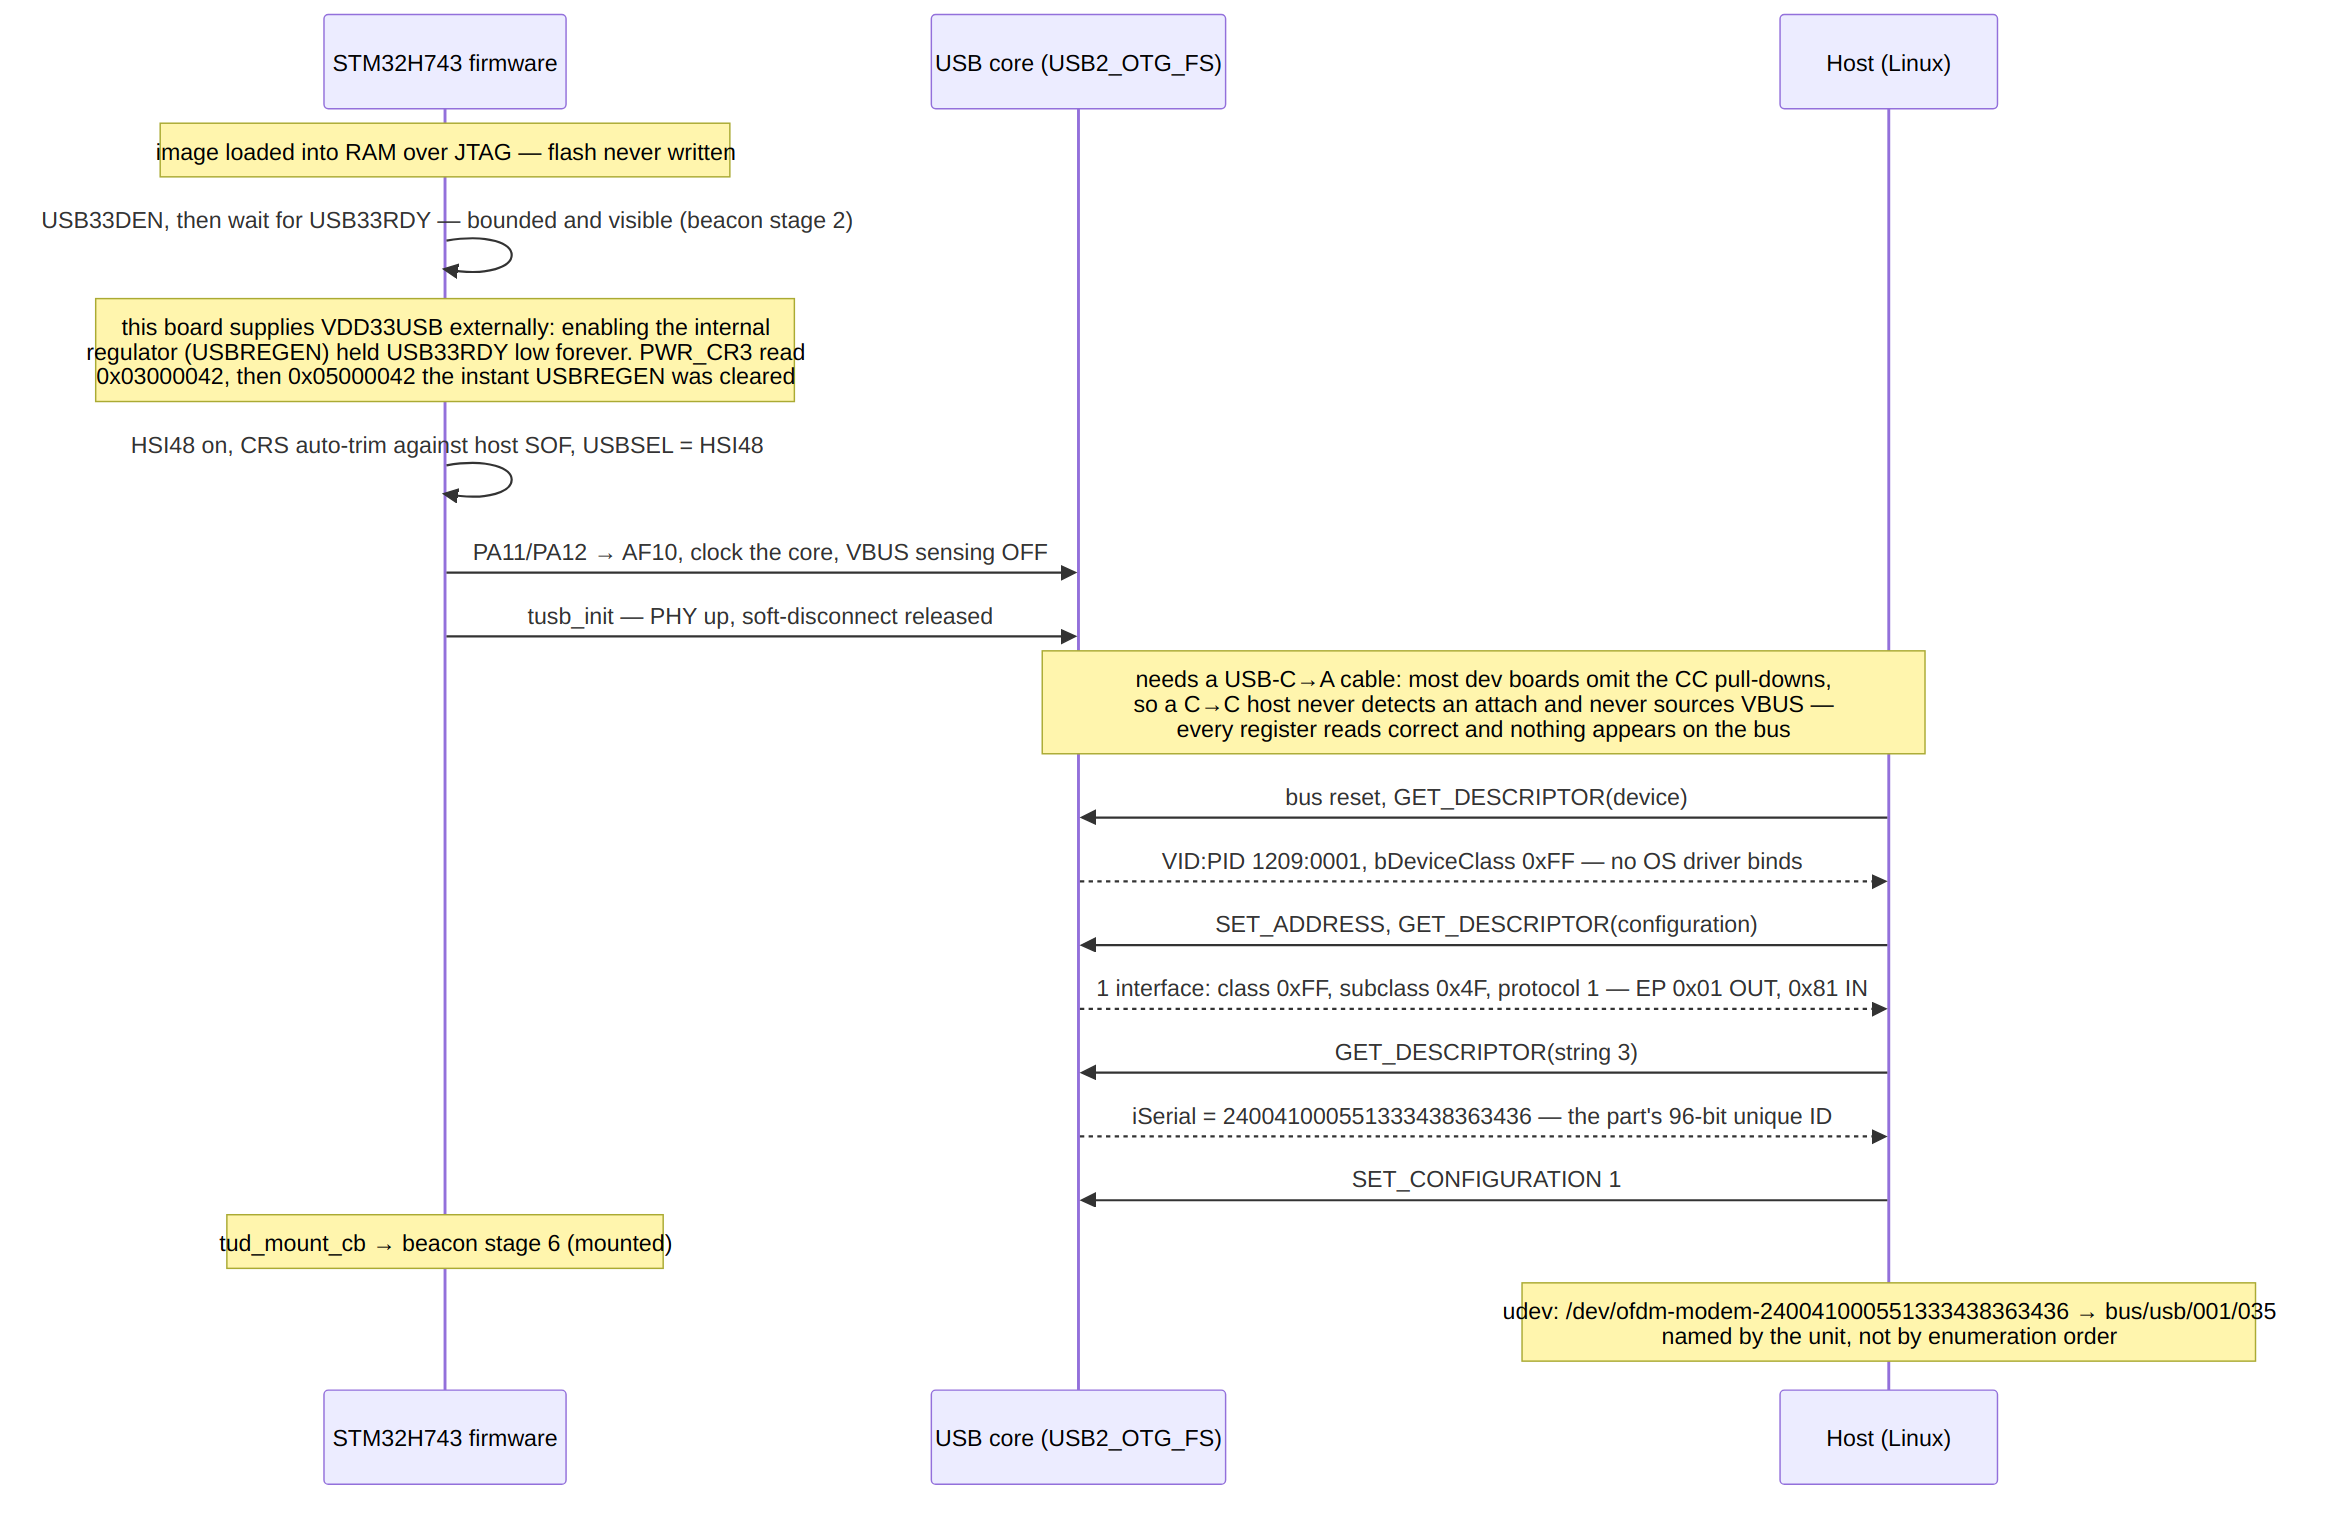
\includegraphics[width=0.92\textwidth]{images/usb_enum_seq.png}
    \caption{Enumeration: supply detection, clocks from HSI48 (trimmed
             against the host's SOF, so the firmware is correct whatever
             the board's crystal), and the descriptors that give the
             device its identity.}
    \label{fig:usbenum}
\end{figure}

\paragraph{A session.} Figure~\ref{fig:usbsession} traces a host
session against the real link layer: the station's queues, rate ladder
and reply timers run for real behind the endpoints, with a stub PHY that
accounts air time and transmits nothing --- the honest shape of a modem
with its antenna disconnected. Status is pushed unprompted twice a
second whenever the device is mounted; the diagnostic event stream is
opt-in and yields to everything else, because a lost diagnostic costs
nothing and a lost reply costs the session.

\begin{figure}[htbp]
    \centering
    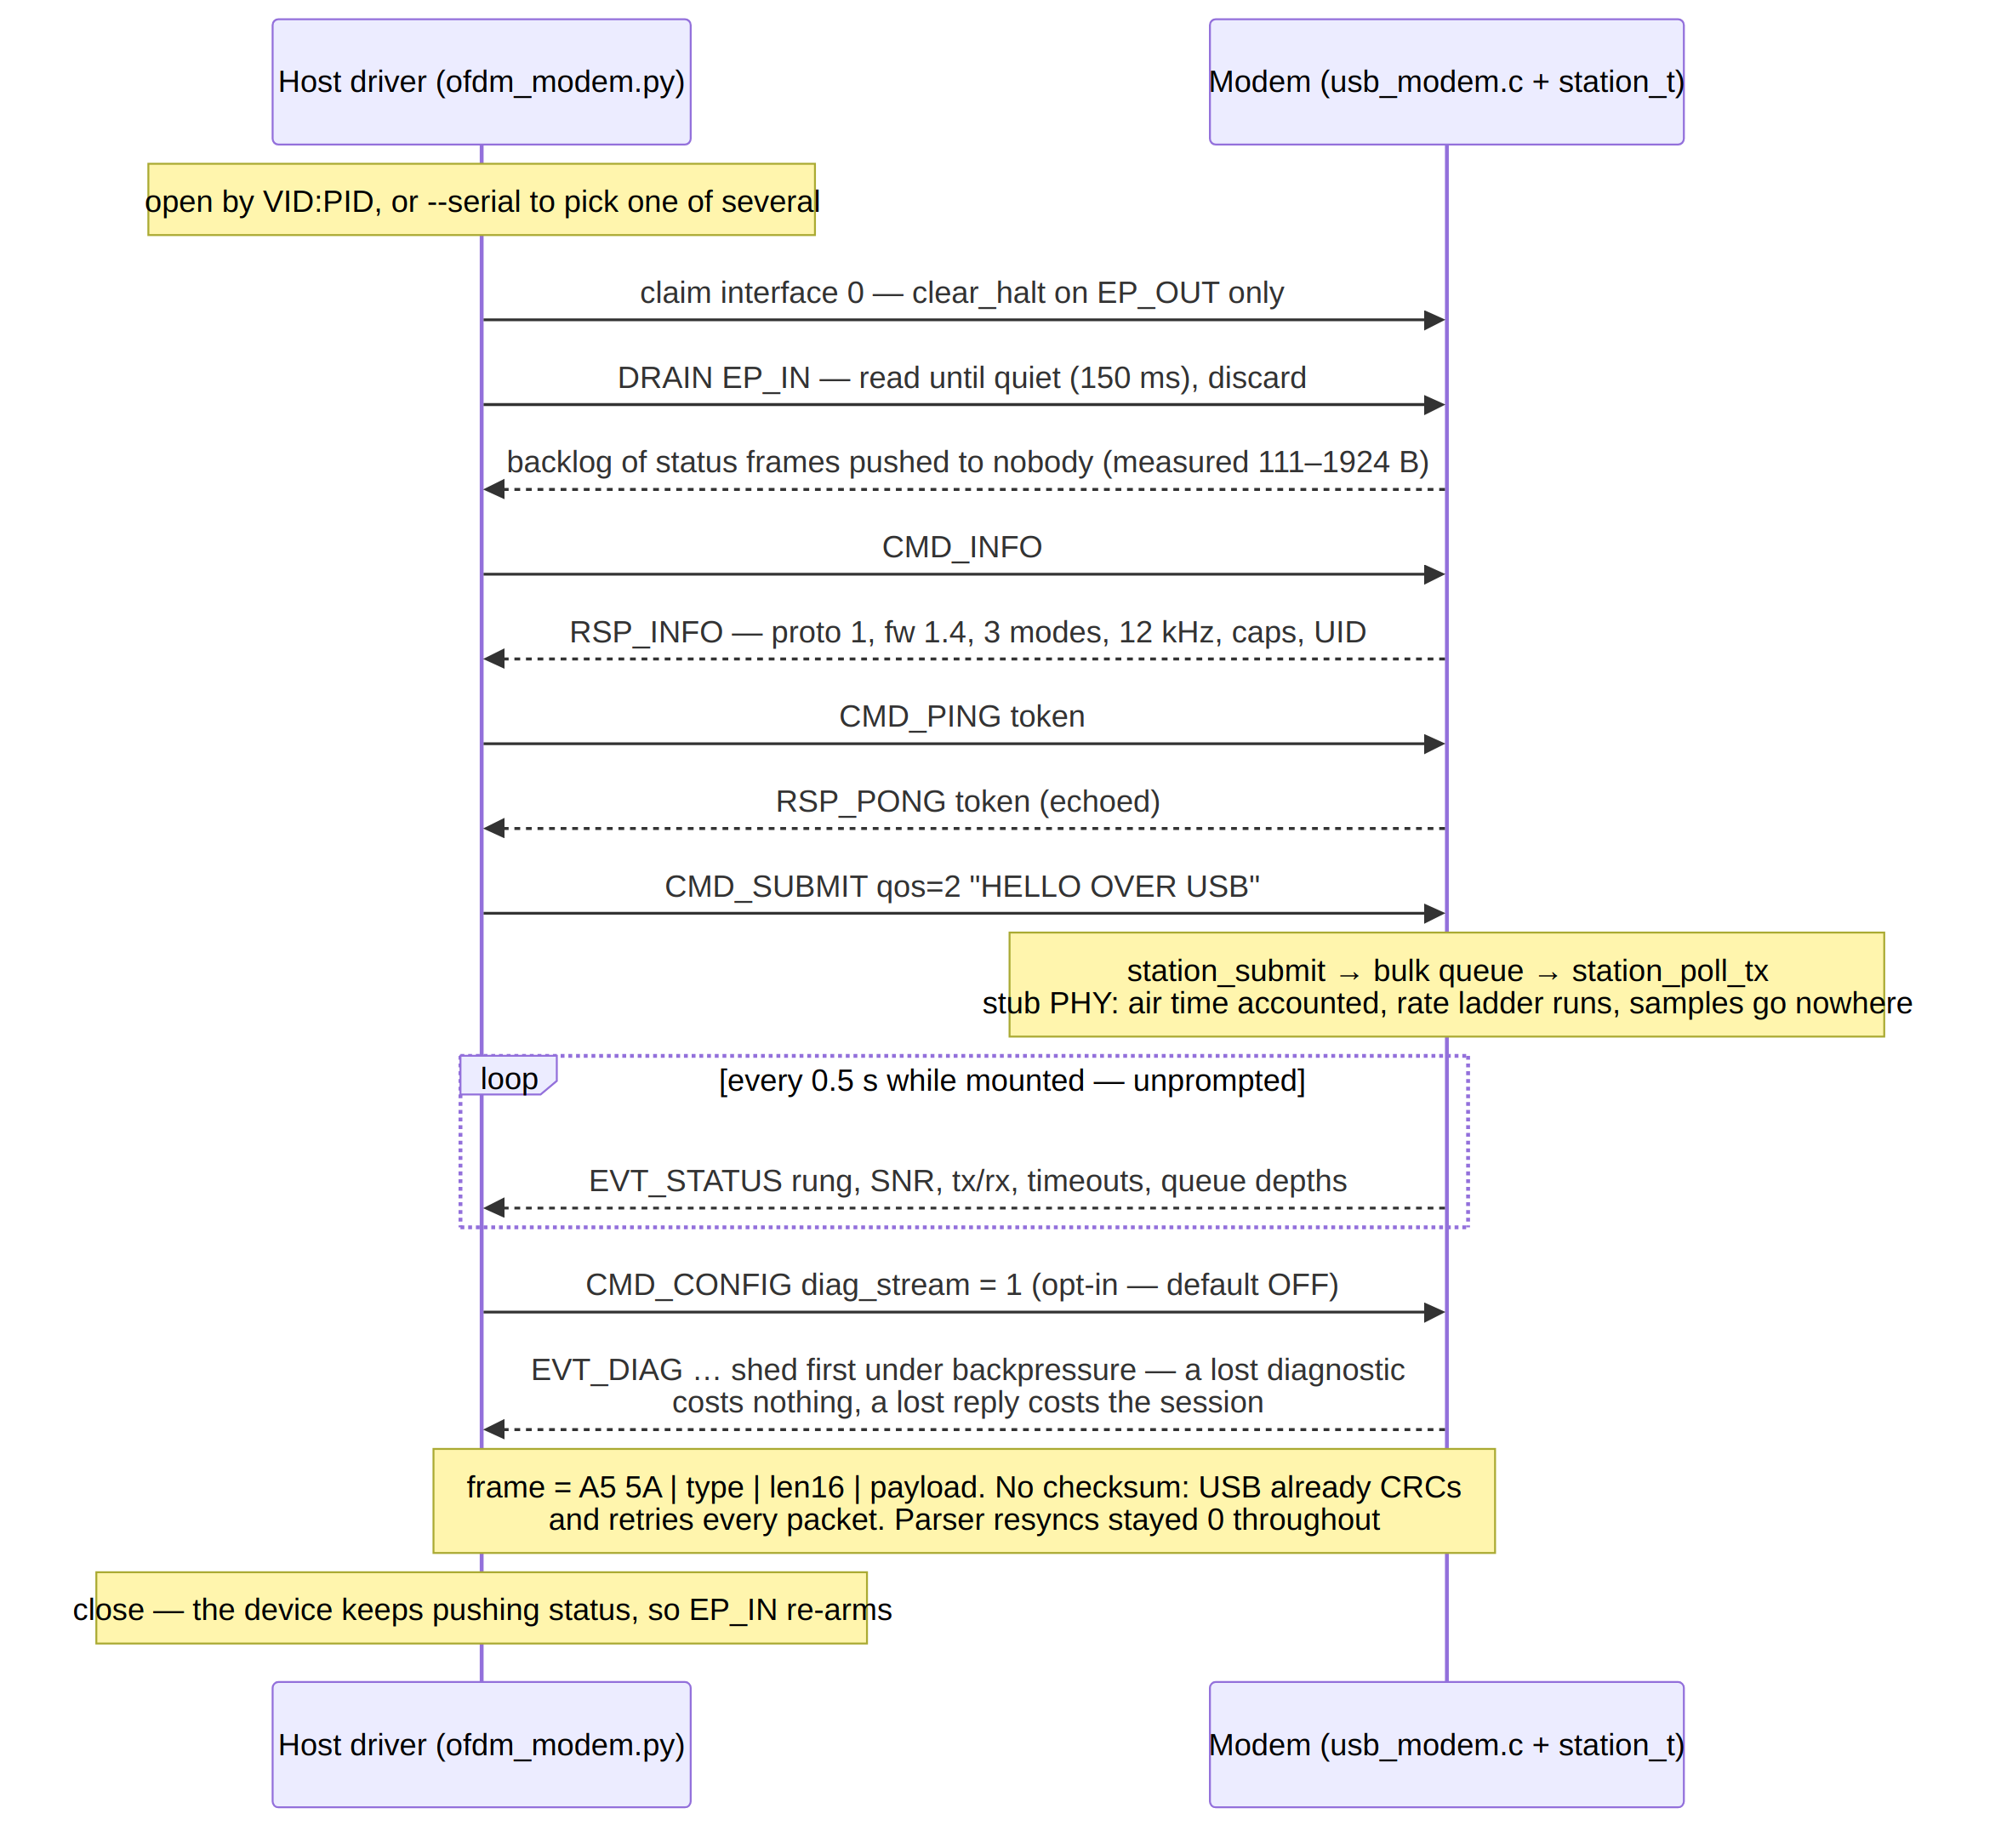
\includegraphics[width=0.92\textwidth]{images/usb_session_seq.png}
    \caption{A host session: open, drain, identify, command and reply,
             unprompted status, opt-in diagnostics.}
    \label{fig:usbsession}
\end{figure}

\paragraph{The wedge, and why the host must drain rather than reset.}
The station image enumerated correctly and then, for most of a day,
answered nothing and fell silent after a single packet --- deterministically,
across four builds. Five hypotheses were disproven by measurement
(a diagnostic firehose, loop starvation under polling, cache against
DMA, polling against interrupts, the clock), and three unrelated bugs
fixed on the way, before the instrumentation at the moment of the stall
read: staging queue empty, 150 bytes free of a 512-byte TinyUSB transmit
FIFO, 399 bytes handed over. That is 362 bytes sitting \emph{inside}
TinyUSB unsent --- 29 (the \texttt{RSP\_INFO} reply) plus nine 37-byte
status frames, exactly --- and $399-362=37$: precisely one frame ever
reached the wire. The device was not silent; it was mute.

The cause, confirmed from TinyUSB's source and shown in
Figure~\ref{fig:usbreopen}, is an interaction between an ordinary host
habit and the library's clear-stall handling. Because the device pushes
status unprompted, its IN endpoint is normally \emph{armed} with a frame
when a host opens it. The host driver called \texttt{clear\_halt} on
that endpoint on open --- a common recovery idiom, and one added during
this work. \texttt{usbd\_edpt\_clear\_stall} drops its software BUSY
flag unconditionally (its own comment calls this ``long-standing
behavior''), while the dwc2 \texttt{dcd\_edpt\_clear\_stall} only clears
the STALL bit and resets the PID; nothing disarms the hardware. The next
flush sees ``not busy'' and re-arms the endpoint on top of a live
transfer --- undefined on the core --- so one packet escapes, the
completion no longer matches what the library started, and BUSY never
clears. The level-triggered FIFO-empty interrupt then storms:
\texttt{isr\_count} reached 90 million.

It was confirmed by prediction rather than by fix. Holding status frames
until the host had spoken, so the endpoint was idle at open, made the
\emph{first} open work --- and every later open still wedged, exactly as
the mechanism requires, since by then the device was pushing again.

The fix is on the host: consume the armed transfer instead of resetting
the endpoint. The driver reads the IN endpoint with short timeouts until
it goes quiet and discards what it finds; \texttt{clear\_halt} is kept
for the OUT endpoint only, where three opens against an armed endpoint
measured harmless. The device is unchanged --- pushing status while
mounted is the right thing for a modem to do, and is the case a driver
must handle. Verified on the part: three consecutive opens (draining
1924, 185 and 111 stale bytes) and a session killed mid-read then
reopened (draining 37 bytes: the one frame armed at the kill), all
answering, submitting and reading with zero resynchronisations;
\texttt{isr\_count} 293 against 90 million wedged, no faults, no drops.

\begin{figure}[htbp]
    \centering
    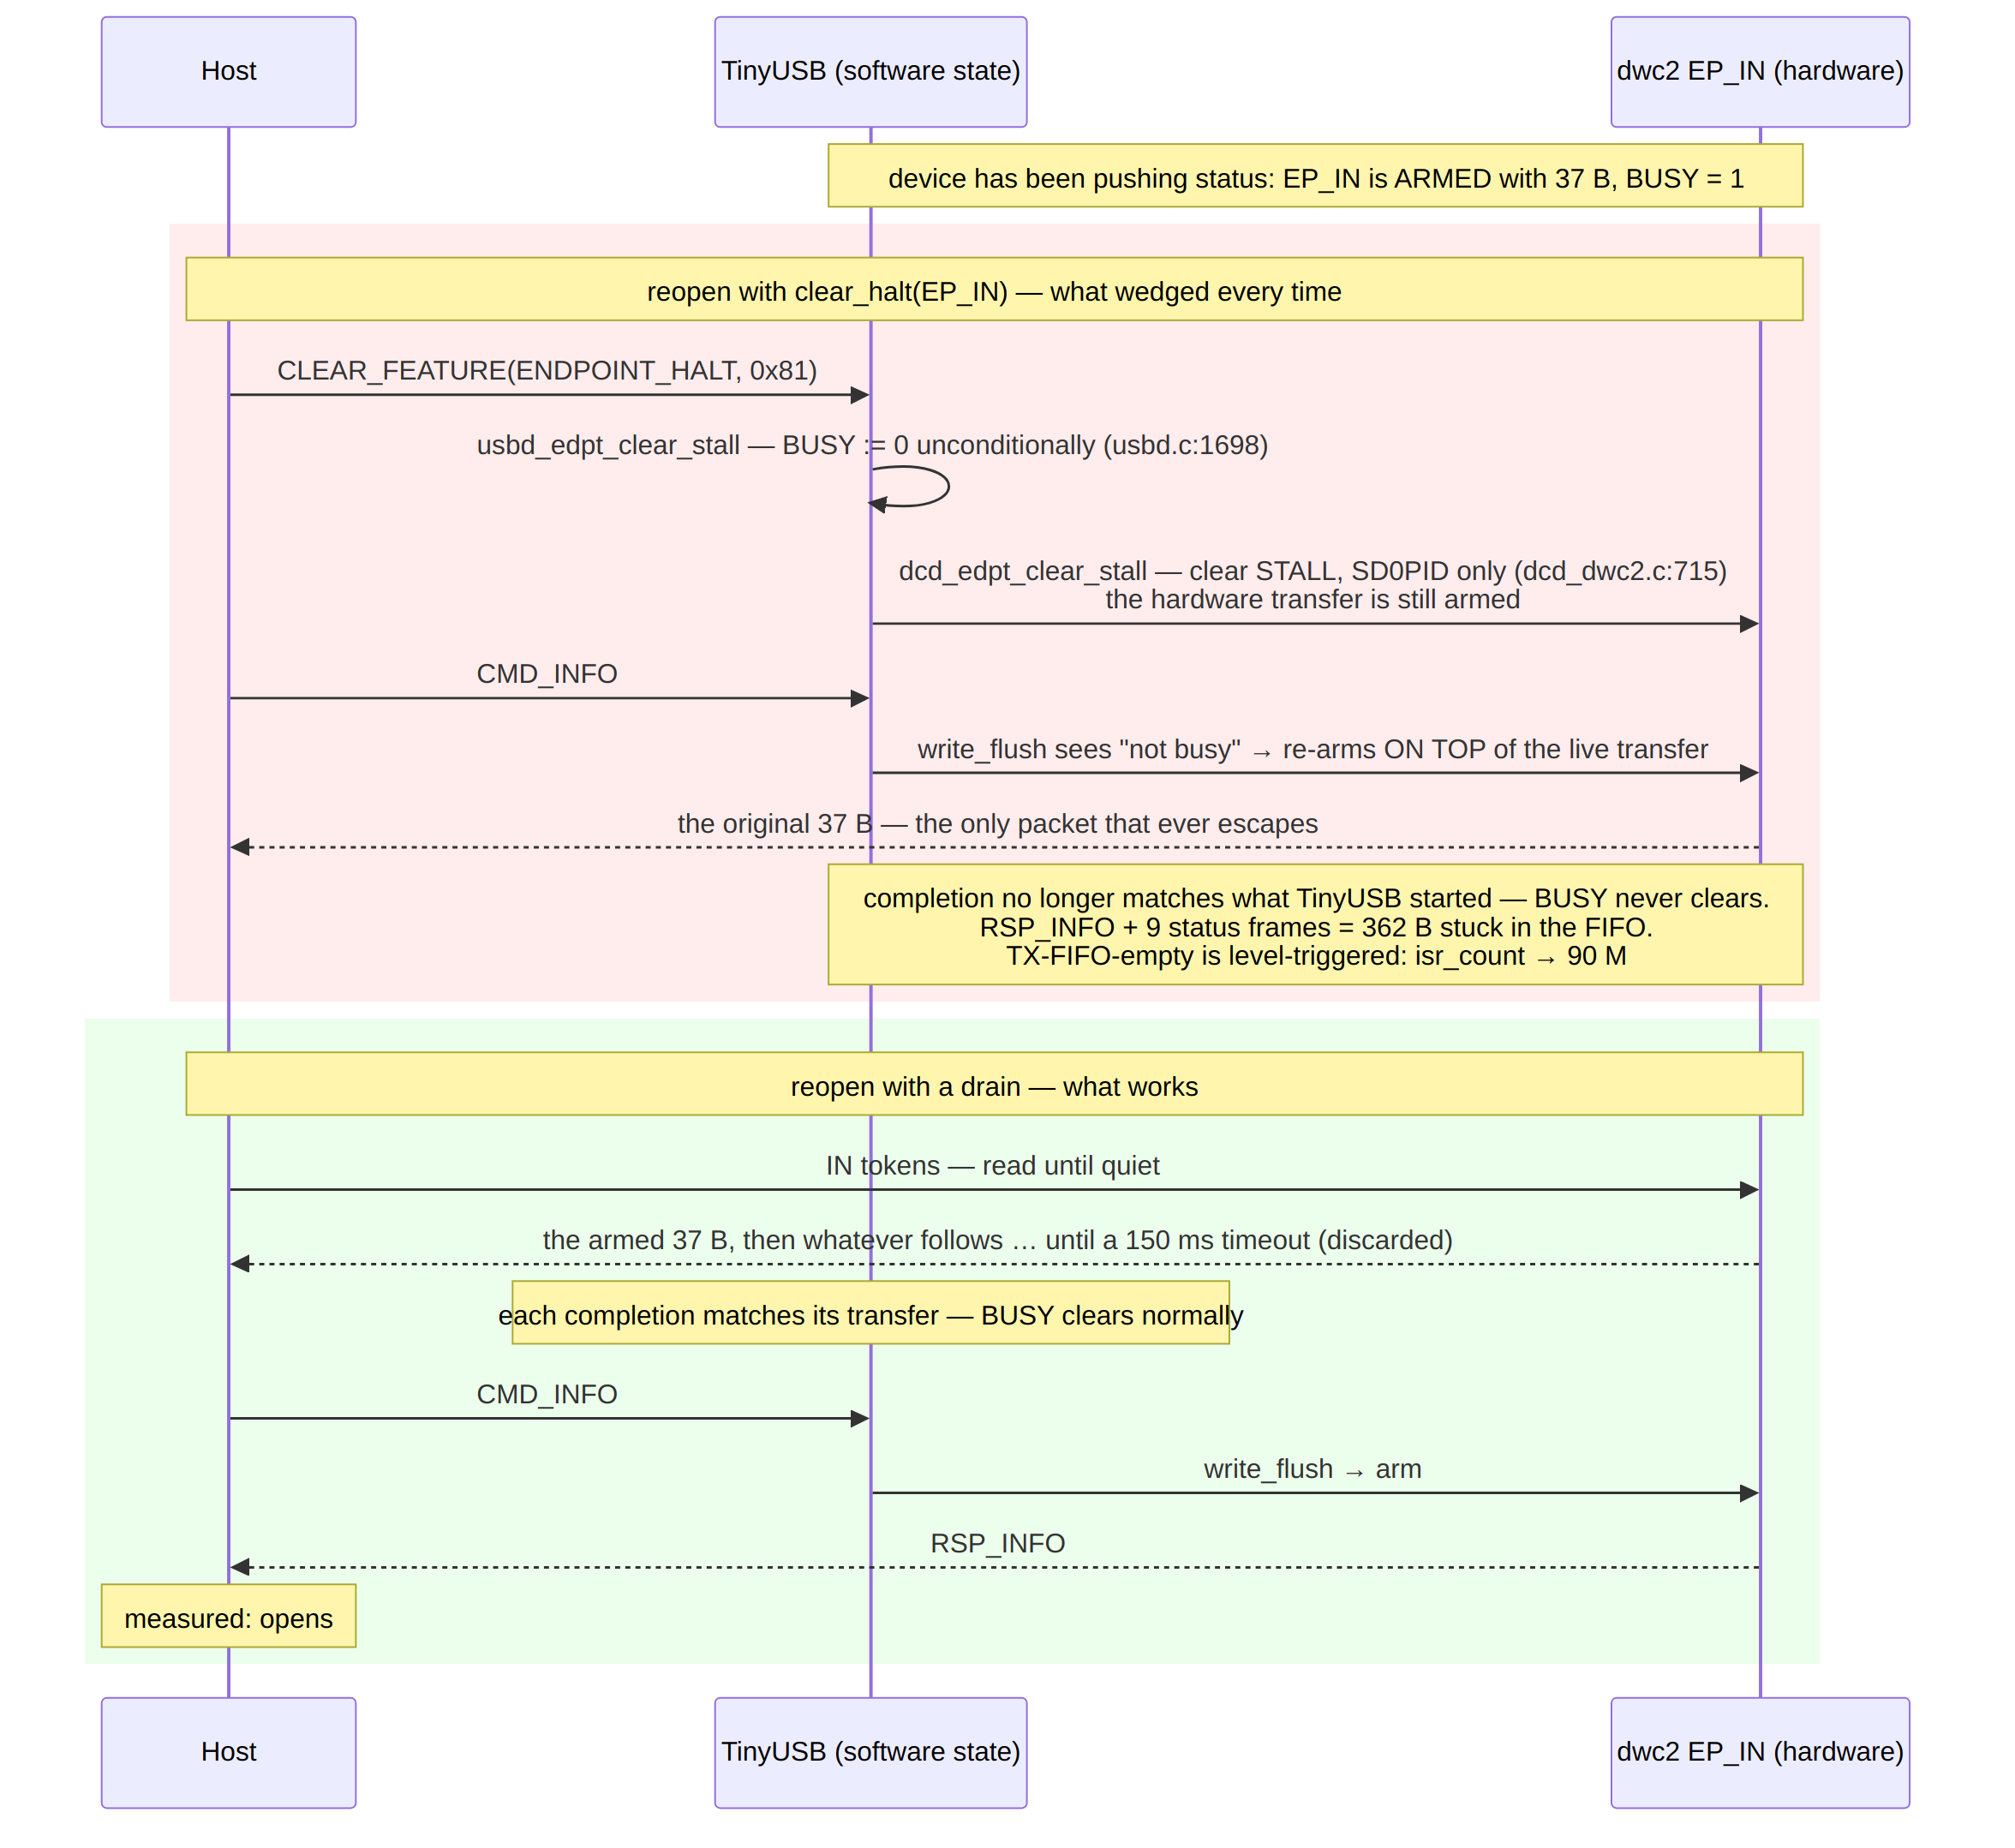
\includegraphics[width=0.92\textwidth]{images/usb_reopen_seq.png}
    \caption{Reopening against a device that is already pushing. Above:
             \texttt{clear\_halt} on an armed IN endpoint desynchronises
             TinyUSB's software state from the hardware and wedges it
             after one packet. Below: draining the endpoint consumes the
             armed transfer through the normal path.}
    \label{fig:usbreopen}
\end{figure}

Two qualifications. VID:PID \texttt{1209:0001} is the pid.codes
\emph{test} identifier, correct for development and wrong for anything
shipped: a released unit needs an allocated product ID, or it collides
with every other prototype using the same one. And the device has not
been made robust to \texttt{clear\_halt} on an armed endpoint itself;
that is TinyUSB's clear-stall path rather than this project's, so the
contract is stated instead --- any client for this device must drain,
not reset.

\subsection{Two Boards on a Wire}
\label{sec:cport_twoboard}

Everything to this point validated the chain against something the
project itself controls: golden vectors, a simulated channel, a virtual
audio daemon, and an SDR whose transmit and receive halves share one
oscillator. One impairment was never exercised by any of them --- two
\emph{independent} clocks. A single-board loopback cannot supply it
either: playing to \texttt{DAC1\_OUT1} and recording \texttt{ADC1} on
the same board runs both converters off one TIM6, so the sample-rate
offset is exactly zero by construction, and the receiver's tolerance to
it is untested no matter how much copper the signal crosses.

The stand in Figure~\ref{fig:twoboardlink} removes that last shared
assumption. Board A's DAC drives board B's ADC through one signal wire
and one ground wire; each board clocks its converter from its own
crystal and its own PLL, and the two never exchange a timing signal ---
not even to start. One ESP32 debugs both boards at once: JTAG
daisy-chains, so \texttt{TDI}/\texttt{TDO} thread through board A into
board B and back to the probe, which costs exactly one wire beyond a
second board's worth of the existing harness. The three push-pull
control lines are duplicated onto a driver pin per board rather than
spliced; because a line and its copy sit in the same GPIO bank, the
firmware switches both in one \texttt{w1ts}/\texttt{w1tc} store, so
there is no skew between the boards at all. That is a wiring
convenience rather than a fix: at the probe's measured 42\,236 edges/s
a TCK half-period is 25\,\textmu s, against nanoseconds of everything
else.

\begin{figure}[htbp]
    \centering
    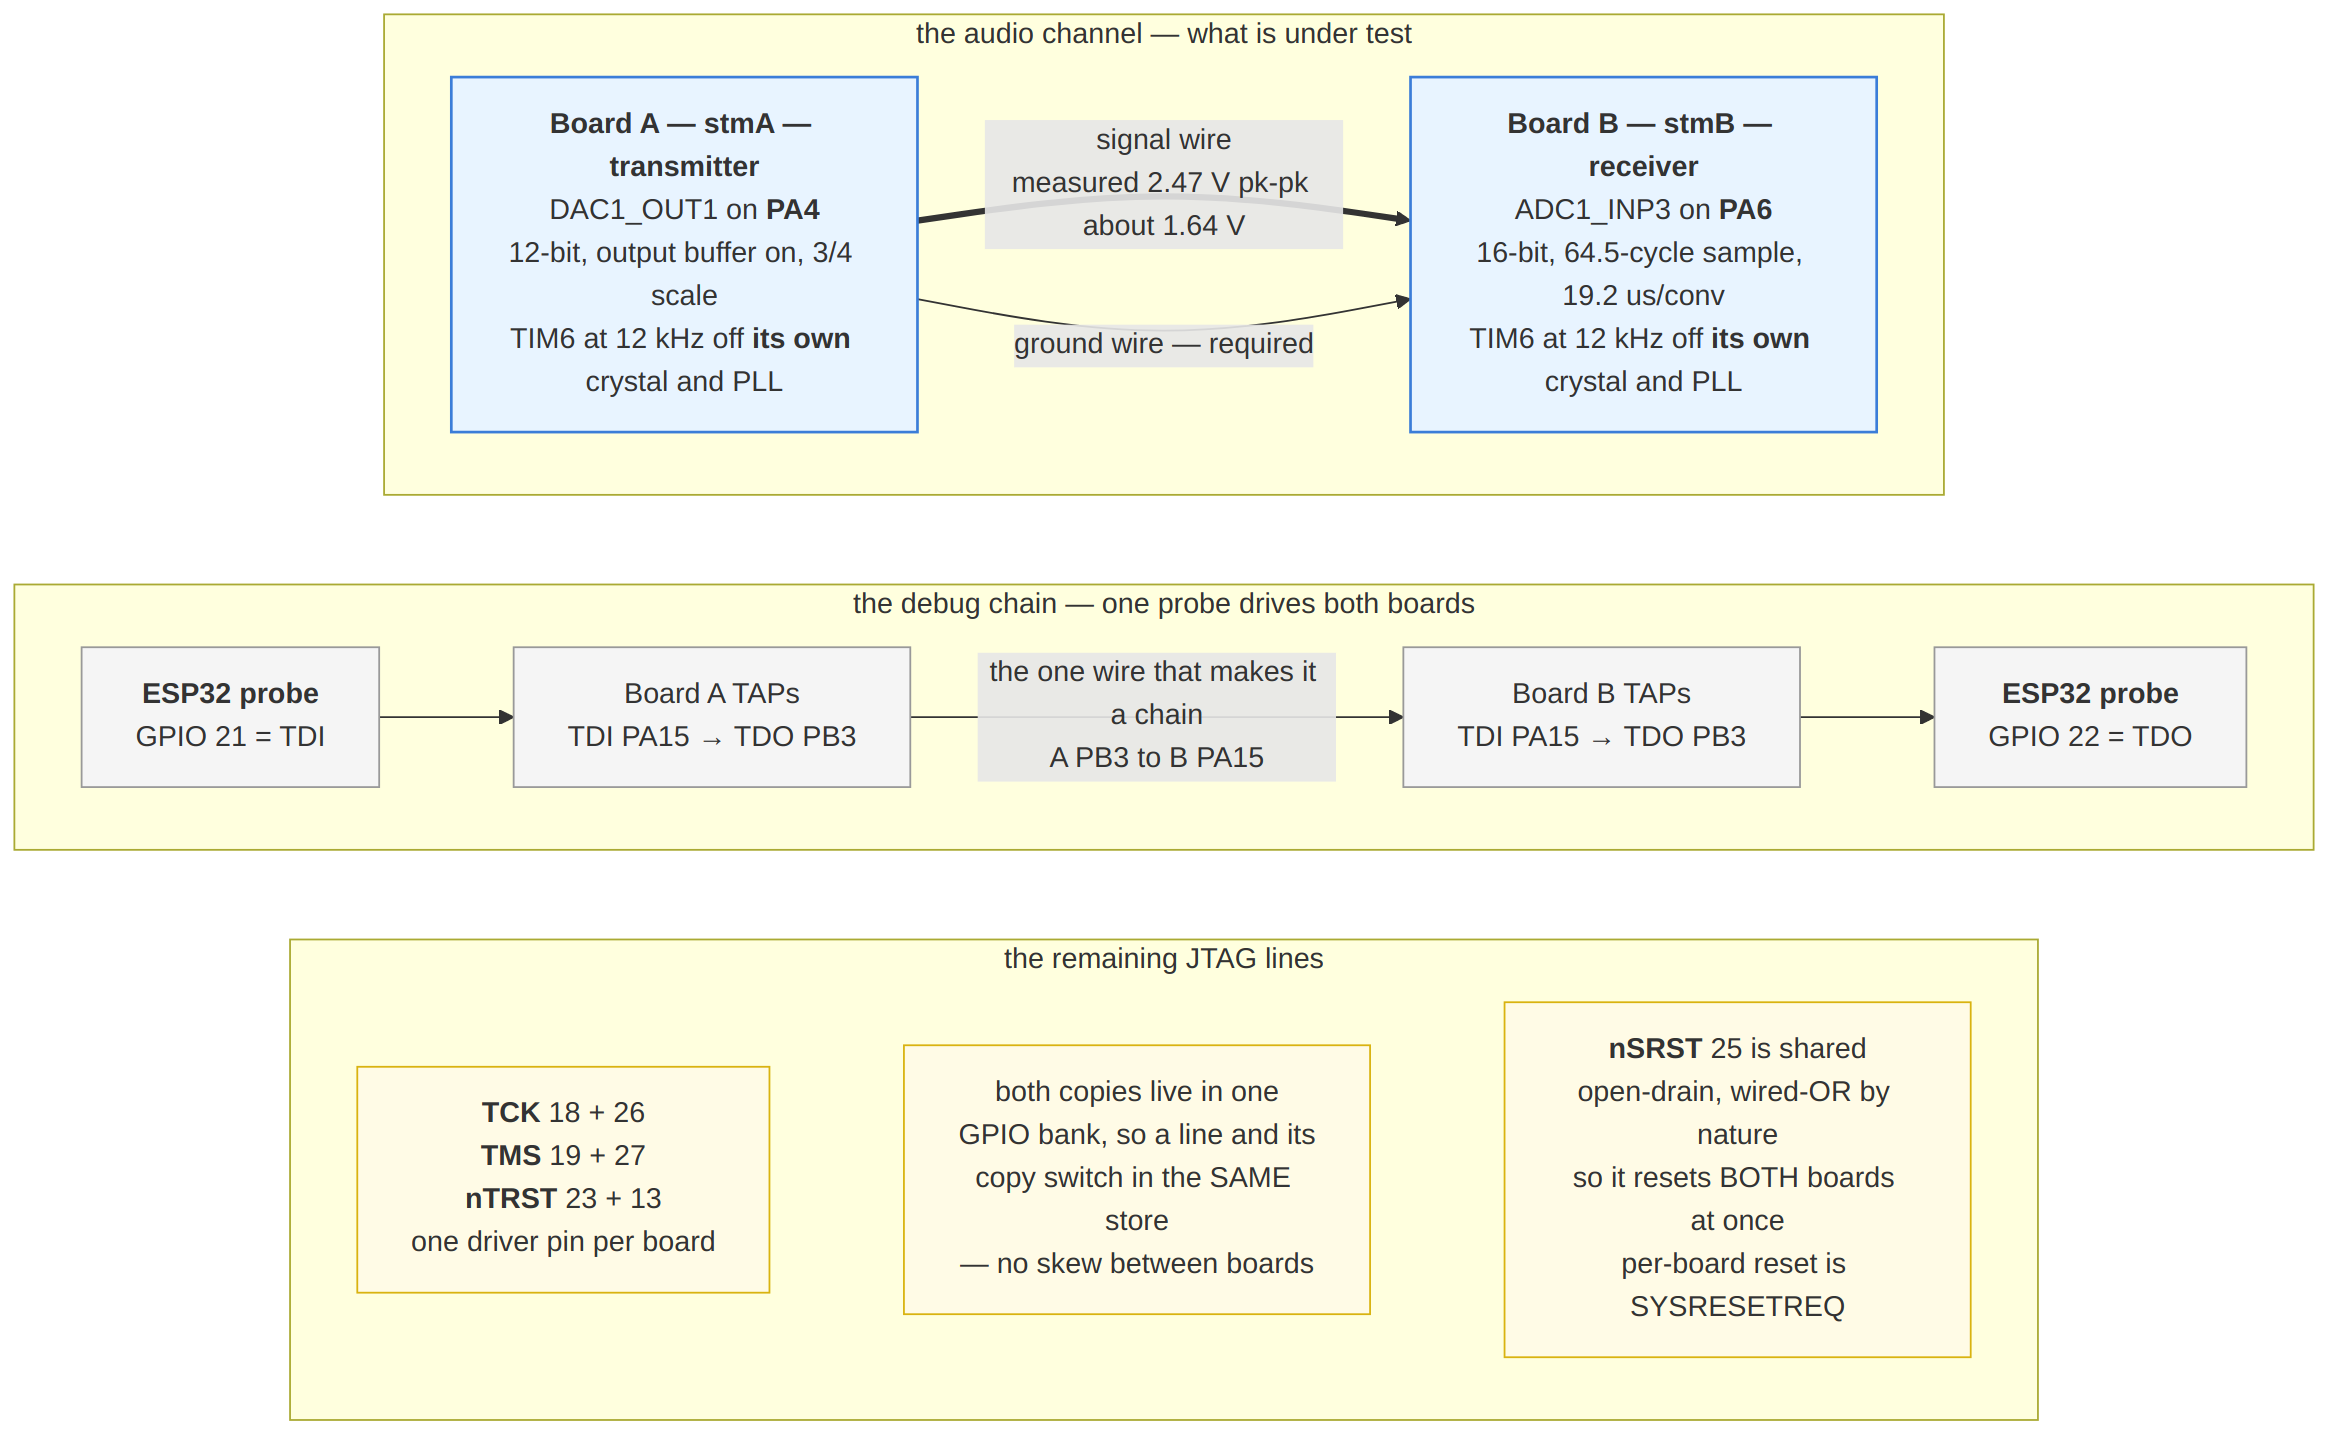
\includegraphics[width=\textwidth]{images/two_board_link.png}
    \caption{The two-board stand. The audio channel is one signal wire
             and one ground wire between converters that share no clock;
             the debug chain is a single probe threaded through both
             boards' TAPs. \texttt{nSRST} is deliberately not
             duplicated --- it is open-drain and wired-OR by nature, and
             duplicating it would not buy per-board reset anyway, since
             \texttt{remote\_bitbang} drives both resets from one pair of
             commands.}
    \label{fig:twoboardlink}
\end{figure}

One image serves both roles, selected over JTAG before the CPU is
released, because a station is half duplex and its transmitter shares
the receiver's arena --- no board ever does both. The transmitter builds
one NORMAL QPSK frame and replays it; the receiver records 54\,000
samples and only then runs the streaming receiver over the recording, so
the analog path can be characterised independently of whether the
decoder liked it. The host releases the transmitter \emph{first}, which
is what removes the need for a trigger: the whole capture window falls
inside a transmission already in progress.

\begin{table}[H]
    \centering
    \caption{Two boards, one wire, independent clocks. Measured on the
             stand; the payload check is \texttt{memcmp} against the
             transmitted packet, so ``bit-exact'' is exact.}
    \label{tab:twoboard}
    \small
    \begin{tabular}{@{}lll@{}}
    \toprule
    \textbf{Quantity} & \textbf{Measured} & \textbf{Note} \\
    \midrule
    Complete frames in window & 2 & 54\,000 samples at 12\,kHz \\
    Decoded bit-exact         & \textbf{2 of 2} & \texttt{memcmp} vs.\ the
                                                  transmitted packet \\
    ADC swing                 & 2.472\,V pk-pk & about 1.643\,V, the
                                                 DAC's mid-rail \\
    Residual CFO              & $+0.01$\,Hz & after preamble correction \\
    ADC conversion            & 19.2\,\textmu s & 64.5-cycle sample,
                                                  \texttt{per\_ck}/8 \\
    Receiver ISR              & 19.5\,\textmu s & of an 83.3\,\textmu s
                                                  period, i.e.\ 23\,\% \\
    Transmitter ISR           & 0.11\,\textmu s & one DAC store \\
    \bottomrule
    \end{tabular}
\end{table}

\paragraph{What it corrected: a vector table in cached SRAM.} The
receiver role hung on its first run --- stage ``running'', its TIM6
interrupt count stuck at zero, the run loop spinning until the
three-minute timeout. The state read off the part was contradictory:
TIM6 counting with its update flag set, the interrupt \emph{pending}
(\texttt{ISPR1}~$=$~\texttt{0x400000}) but \emph{not enabled}
(\texttt{ISER1}~$=$~0), \texttt{PRIMASK} clear --- and the vector table
in memory holding the correct handler. The status block explained the
disable: the first interrupt had been taken by the \emph{stray} handler,
whose job is to mask an unexpected source rather than let it wedge the
device, so it had cleared the enable for IRQ~54.

The vector table lives in ordinary cached SRAM, and
\texttt{vectors\_set()} wrote the entry and executed \texttt{DSB} ---
which orders accesses but does not clean. On a Cortex-M7 an exception
vector fetch reads \emph{memory}, not the D-cache, so the new entry sat
in a dirty line while the hardware still fetched the old one. Reading
the table over JTAG showed the correct handler only because the line had
been evicted by then, which is precisely what made the failure look
impossible. \texttt{SCB\_CCR} read \texttt{0x00070200} on the stalled
board, \texttt{DC} set --- inherited from the USB firmware the RAM image
had displaced. The transmitter role never hit it because
\texttt{build\_frame()} runs between installing the handler and the
first interrupt and evicts the line in time: the same binary on the same
board, differing only in eviction timing, which is why the bug presented
as role-dependent. Both entry points now clean by MVA. This had been
latent under every RAM bench in the project.

Two smaller hazards came from the same root --- a RAM image inherits the
machine state of the firmware it replaced. \texttt{ISER3} bit~5
(\texttt{OTG\_FS}) is still set when the image starts, so an inherited
enable can deliver a stale interrupt as the first one and get its source
masked; \texttt{vectors\_irq\_enable()} therefore clears the pending bit
before setting the enable, and the bench masks interrupts for the whole
of bring-up.

\paragraph{What was not measured.} The obvious way to report the
sample-rate offset --- compare the two boards' measured TIM6 clocks ---
is structurally incapable of showing it, and would have produced a
confident \emph{0.0\,ppm}. Each board measures TIM6 against its own DWT
cycle counter, and both are derived from the \emph{same} PLL, so that
ratio is exact on each board and identical between them however far
apart the crystals are. The offset is instead read off the wire, from
the spacing of consecutively decoded frames against the number of
samples transmitted between them. With only two complete frames in the
capture window the span is 17\,920 samples, and a start position good to
one sample makes that a \emph{bound} rather than a figure: the two
clocks agree to within $\pm$56\,ppm. That is consistent with the
$+0.01$\,Hz residual CFO, and it is enough to say the link decodes
across independent clocks --- but it is not a measurement of their
offset. A tighter number needs a much longer capture, which needs the
receiver to decode as it goes rather than into a buffer; that is the
next step for this stand, not a result of it.

\subsection{A Board That Is a Radio}
\label{sec:cport_radio}

Section~\ref{sec:cport_usb} gave the board an identity and a host
protocol, but bound the station to a \emph{stub} PHY: queues, rate
ladder, ARQ and reply timers all ran for real, and nothing reached the
air. Section~\ref{sec:cport_twoboard} gave the opposite half --- frames
crossing copper between two boards' converters --- with no link layer
above them and no host beside them. This section is the two in one
image: a board a host drives over USB and a peer hears over a wire.

\begin{figure}[htbp]
    \centering
    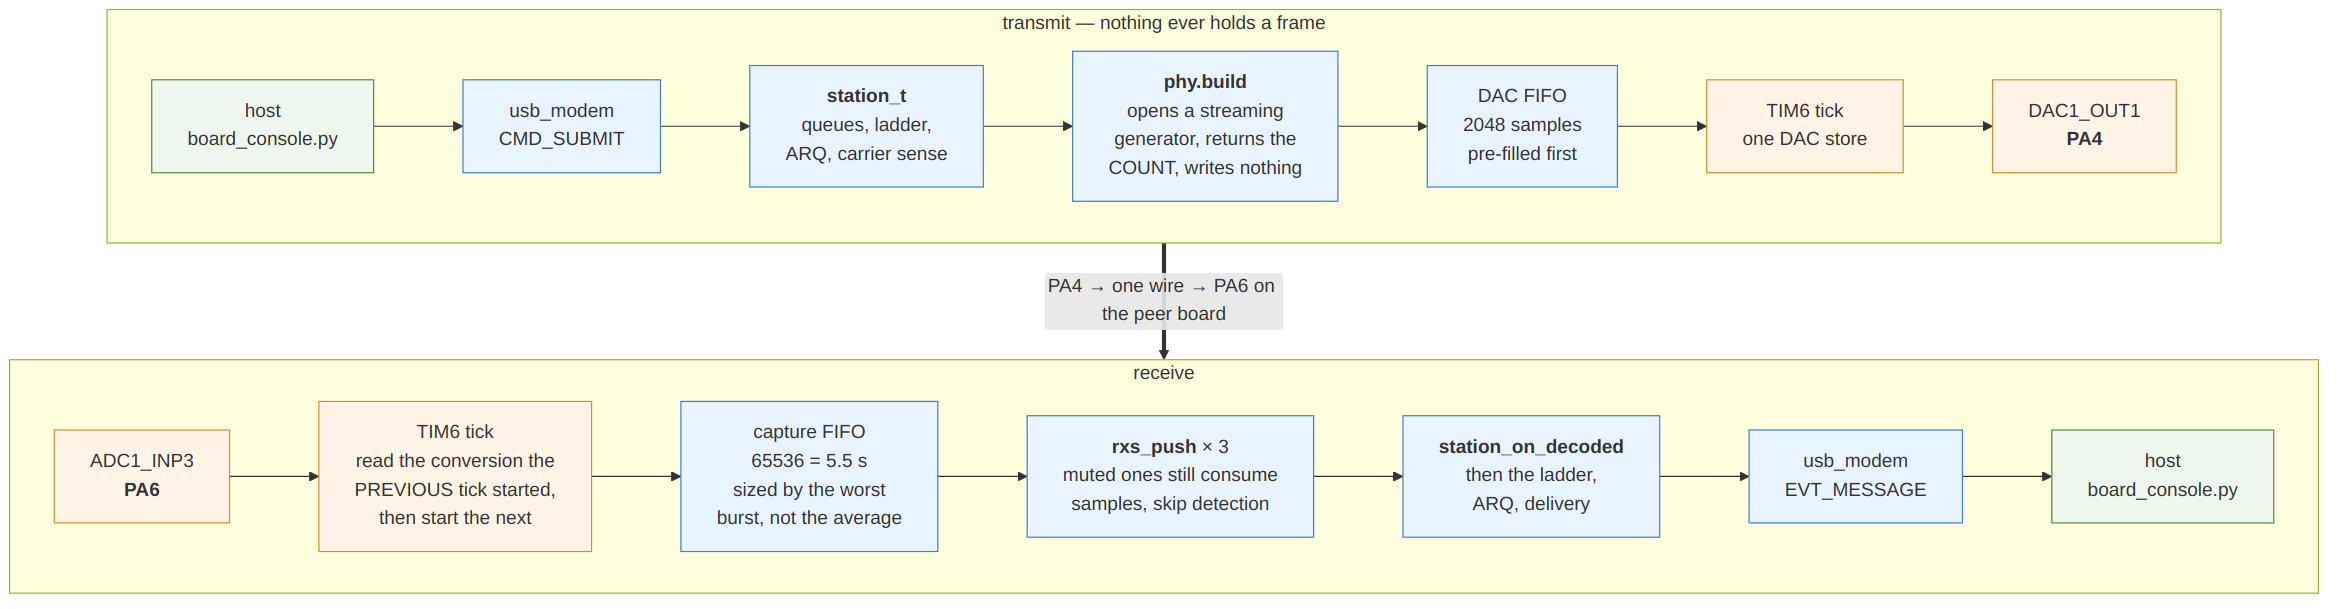
\includegraphics[width=\textwidth]{images/radio_firmware.png}
    \caption{The radio firmware. Half duplex here is a contract rather
             than a simplification: the streaming generator's state
             lives in the shared arena \emph{across} \texttt{txs\_pull}
             calls while the receiver's scratch is call-scoped, so
             \texttt{rxs\_push} must never run during a transmission ---
             and does not, because the tick feeds only one FIFO at a
             time.}
    \label{fig:radiofw}
\end{figure}

\paragraph{The transmitter never renders a frame.}
\texttt{station\_phy\_t::build} is frame-at-once: it is handed a buffer
and returns a sample count. An EXTREME frame is about 456\,000 samples
--- 912\,kB --- which this part cannot hold, and demoapp's answer (a
600\,000-sample buffer) is not available. It is also unnecessary. The
station never reads or writes those samples: \texttt{out} and
\texttt{out\_cap} appear nowhere in \texttt{station\_poll\_tx} except
where they are passed through to \texttt{build}, and the count is what
the caller acts on. So \texttt{build} here opens a \emph{streaming}
generator and returns the total it reports without writing a sample,
and the main loop pulls from that generator into a 2048-sample FIFO as
the tick drains it. The waveform is identical either way --- a one-block
burst with no resync is bit-for-bit a frame, which both test suites
already assert.

The 12\,kHz tick never blocks. The analog bench of
Section~\ref{sec:cport_twoboard} started a conversion and waited for it
inside the tick, 19.2\,\textmu s of an 83.3\,\textmu s period; that was
free when the decoder ran afterwards and is not free when the decoder
has to keep up. Here the tick reads the conversion the \emph{previous}
tick started and immediately starts the next, so the sample is one tick
old --- a constant delay indistinguishable from cable length.

\paragraph{What it corrected: the flash images never enabled the
caches.} The receiving board dropped 1\,522\,686 captured samples ---
64\,\% of everything its ADC produced --- and decoded nothing, while the
transmitting board underran its DAC 375 times. \texttt{SCB\_CCR} read
\texttt{0x00040200} on the running part: both L1 caches off.
\texttt{startup\_flash.c} had never enabled them, so code ran from flash
at two wait states with no instruction cache and every SRAM access
uncached, which is five to ten times slower than the same code out of
ITCM. It had not mattered while the flash images only ran a USB endpoint
and a link layer, and the RAM benches never showed it because their
\texttt{.text} lives in ITCM and needs no cache. Enabling both (the data
cache invalidated by set/way first) cut overruns by 61$\times$. Two
consequences follow and are handled rather than discovered later: a
debugger reading over the AHB-AP does \emph{not} see dirty lines, so the
beacon is cleaned explicitly before each read; and a RAM image that now
inherits \texttt{DC}=1 needs its vector-table writes cleaned, which is
what Section~\ref{sec:cport_twoboard} already had to fix.

Three smaller faults surfaced with it. The flash linker script listed
\texttt{.bss} \emph{before} \texttt{.d2\_bss}, and \texttt{.bss}'s
\texttt{*(.bss*)} matches \texttt{.bss.g\_raw} too --- so the D2 lines
matched nothing, the 160\,kB sample ring sat in AXI, and adding the
receiver overflowed AXI by 100\,kB while D2 stood completely empty
(\texttt{stm32h743\_usb.ld} always had the right order, which is why only
the flash images were affected). \texttt{TIM6\_DAC}, IRQ~54, had no entry
in the vector table: designated initialisers leave every other slot
\texttt{NULL}, so the first tick would have vectored to address zero.
And arming an empty DAC FIFO underran it once per transmission ---
166 underruns across 3 frames, each one a mid-rail sample on the air ---
which pre-filling before starting the carrier reduces to zero.

\paragraph{Sizing the capture FIFO: the worst burst, not the average.}
The decoder's cost is wildly uneven. Quiet blocks are cheap; the commit
at the end of a frame --- acquisition, demodulation of every tiled
symbol, Viterbi --- is one long blocking call, measured at 2283\,ms
inside a single \texttt{rxs\_push} against a 19.5\,s frame. As an
average that is about 12\,\% duty, comfortably real time. What matters
is not the average but whether the FIFO can hold the samples that keep
arriving \emph{through} the burst: 16\,384 samples (1.37\,s) could not,
dropping 33\,036 samples mid-frame and decoding nothing, while 65\,536
(5.5\,s) decodes with no overruns at all. The beacon carries
\texttt{cap\_overruns} and \texttt{push\_ms\_max} so this is checked on
the part rather than reasoned about.

\paragraph{The receiver follows the negotiated rung.} Each open receiver
runs its own detector over every sample and the EXTREME one is much the
most expensive; three concurrently do not fit real time on this part.
They cannot simply be opened selectively either, because every instance
shares one raw sample ring and indexes it by its \emph{own} sample
counter --- feed a subset and they write each other's history at the
wrong offsets. So all three are opened and the unwanted ones are
\emph{muted}: a muted instance still consumes every sample, keeping the
ring and its own timeline coherent, and skips only the per-block
detection, which is where the cost is. Unmuting rearms the search rather
than resuming, since a state machine that was mid-frame when it went
quiet would otherwise decode a frame whose middle it never saw.

Which are active follows \texttt{ladder\_mode(ctl.my\_req)} --- the rung
\emph{this} station asked the peer to transmit at --- plus two others
that are not optional. EXTREME always, because it is rung~0 and
therefore the bootstrap, it is where the ladder decays to after a spell
of silence, and it is what a peer that cannot hear us falls back to;
muting it would make the link undiscoverable and unrecoverable exactly
when recovery is needed. And the mode last decoded on, because
\texttt{my\_req} is a request rather than an observation: between raising
it and the peer acting on it, the peer is still transmitting at the old
mode, and dropping that mode immediately would make the station deaf for
precisely the exchange that would have confirmed the change --- timeout,
request decays, link oscillates. In the settled bootstrap state, both
terms are EXTREME and exactly one detector runs.

\begin{table}[H]
    \centering
    \caption{Two boards, one wire, driven from two host consoles. Every
             figure read off the boards' beacons or the consoles.}
    \label{tab:radio}
    \small
    \begin{tabular}{@{}lll@{}}
    \toprule
    \textbf{Quantity} & \textbf{Measured} & \textbf{Note} \\
    \midrule
    First message, end to end & 36\,s & EXTREME bootstrap,
                                        $\approx$19.5\,s of air \\
    Second message            & \textbf{15\,s} & after the ladder
                                                 climbed \\
    Frames / decodes, each board & 1 / 1 & B decoded, replied, A decoded
                                           the reply \\
    Capture overruns          & \textbf{0} & both boards, throughout \\
    DAC underruns             & \textbf{0} & both boards, after
                                             pre-filling \\
    Worst single decode       & 2283\,ms & of a 19.5\,s frame,
                                           $\approx$12\,\% duty \\
    Idle listening set        & EXTREME & \texttt{my\_req} 0, one
                                          detector \\
    After the climb           & NORMAL$+$EXTREME & \texttt{my\_req} 9
                                                   (A), 7 (B) \\
    SNR reported              & $+15.0$ / $+9.7$\,dB & A and B \\
    \bottomrule
    \end{tabular}
\end{table}

What this build does not yet do is decode streamed bursts: it provides
\texttt{build\_burst} but leaves \texttt{receive\_burst} \texttt{NULL},
so the station uses per-frame bursts --- which is a supported
configuration rather than a hole, since it is also where the link falls
back when a stream stops delivering. Streamed reception needs
\texttt{rxs\_continue\_burst} driven from the link layer's marker, as
demoapp does.

\subsection{Demonstration Infrastructure}
\label{sec:cport_demo}

The C stack runs end-to-end in an interactive demonstration
(\texttt{demoapp/}): a virtual channel daemon exposes two station
devices and a configuration device over Unix sockets, moves 12\,kHz
\texttt{int16} audio in paced ticks, and applies propagation delay,
AWGN sized against the delivered-signal RMS, one-pole Rayleigh fading,
and half-duplex muting; an optional audio mode plays each station's
receive signal on one stereo channel with the sound card as the pacing
clock, making the protocol audible (the EXTREME bootstrap's 21-second
warble adapting up to sub-second QAM16 chirps).  Two console station
applications (three streaming receivers each, one per mode, over the
shared ring) provide messaging, multi-part file transfer over the
burst protocol, channel statistics, the diagnostic event stream, and
the oscillator fine-tune command.  A scripted smoke test drives the
whole stack --- text plus a 5\,000-byte file across the impaired
channel, byte-compared on arrival --- at $25\times$ time scale; the
protocol clocks itself from received samples, so behaviour is
identical at any scale.  The stop-and-wait inefficiency, the burst
protocol's window bugs, the carrier-sense threshold and the rung-0
fallback were all found by this infrastructure rather than by
inspection.

Figure~\ref{fig:sendfileseq} traces a file transfer through it.  Two
decisions in that sequence are worth isolating.

The file is deflated \emph{whole} before being split into parts, not
per part: a 14162-byte configuration file becomes 5015 bytes on air
($2.82\times$), and compressing each 3\,kB part separately would throw
most of that away.  Compression lives in the application rather than in
\texttt{cport/}, which keeps the C port dependency-free --- an MCU
build swaps zlib for miniz or heatshrink and the wire format is plain
\textsc{deflate} either way.

The transfer also \emph{negotiates before it commits}.  The transmit
rung decays by one step per 90\,s of peer silence
(Section~\ref{sec:link}), so a transfer started after a quiet
spell would otherwise open at a rung the link has never been tested at:
measured, a 37.0\,s frame at rung~4 immediately before the next
exchange settled at rung~12 and 5.1\,s.  A sub-second control frame is
answered, and an answered frame is what moves the ladder, so the probe
goes first and the bulk queue follows behind it.  The staleness test
must ask whether the peer has \emph{ever} reported rather than
subtracting from the initial timestamp --- the sentinel is
$-10^{9}$, and doing the arithmetic anyway reported that the peer had
last been heard from 1000000058\,seconds ago.  It is the same rule the
link layer already follows for sequence numbers, where every value
0--7 is legitimate and ``nothing yet'' must be its own state.

\begin{figure}[H]
    \centering
    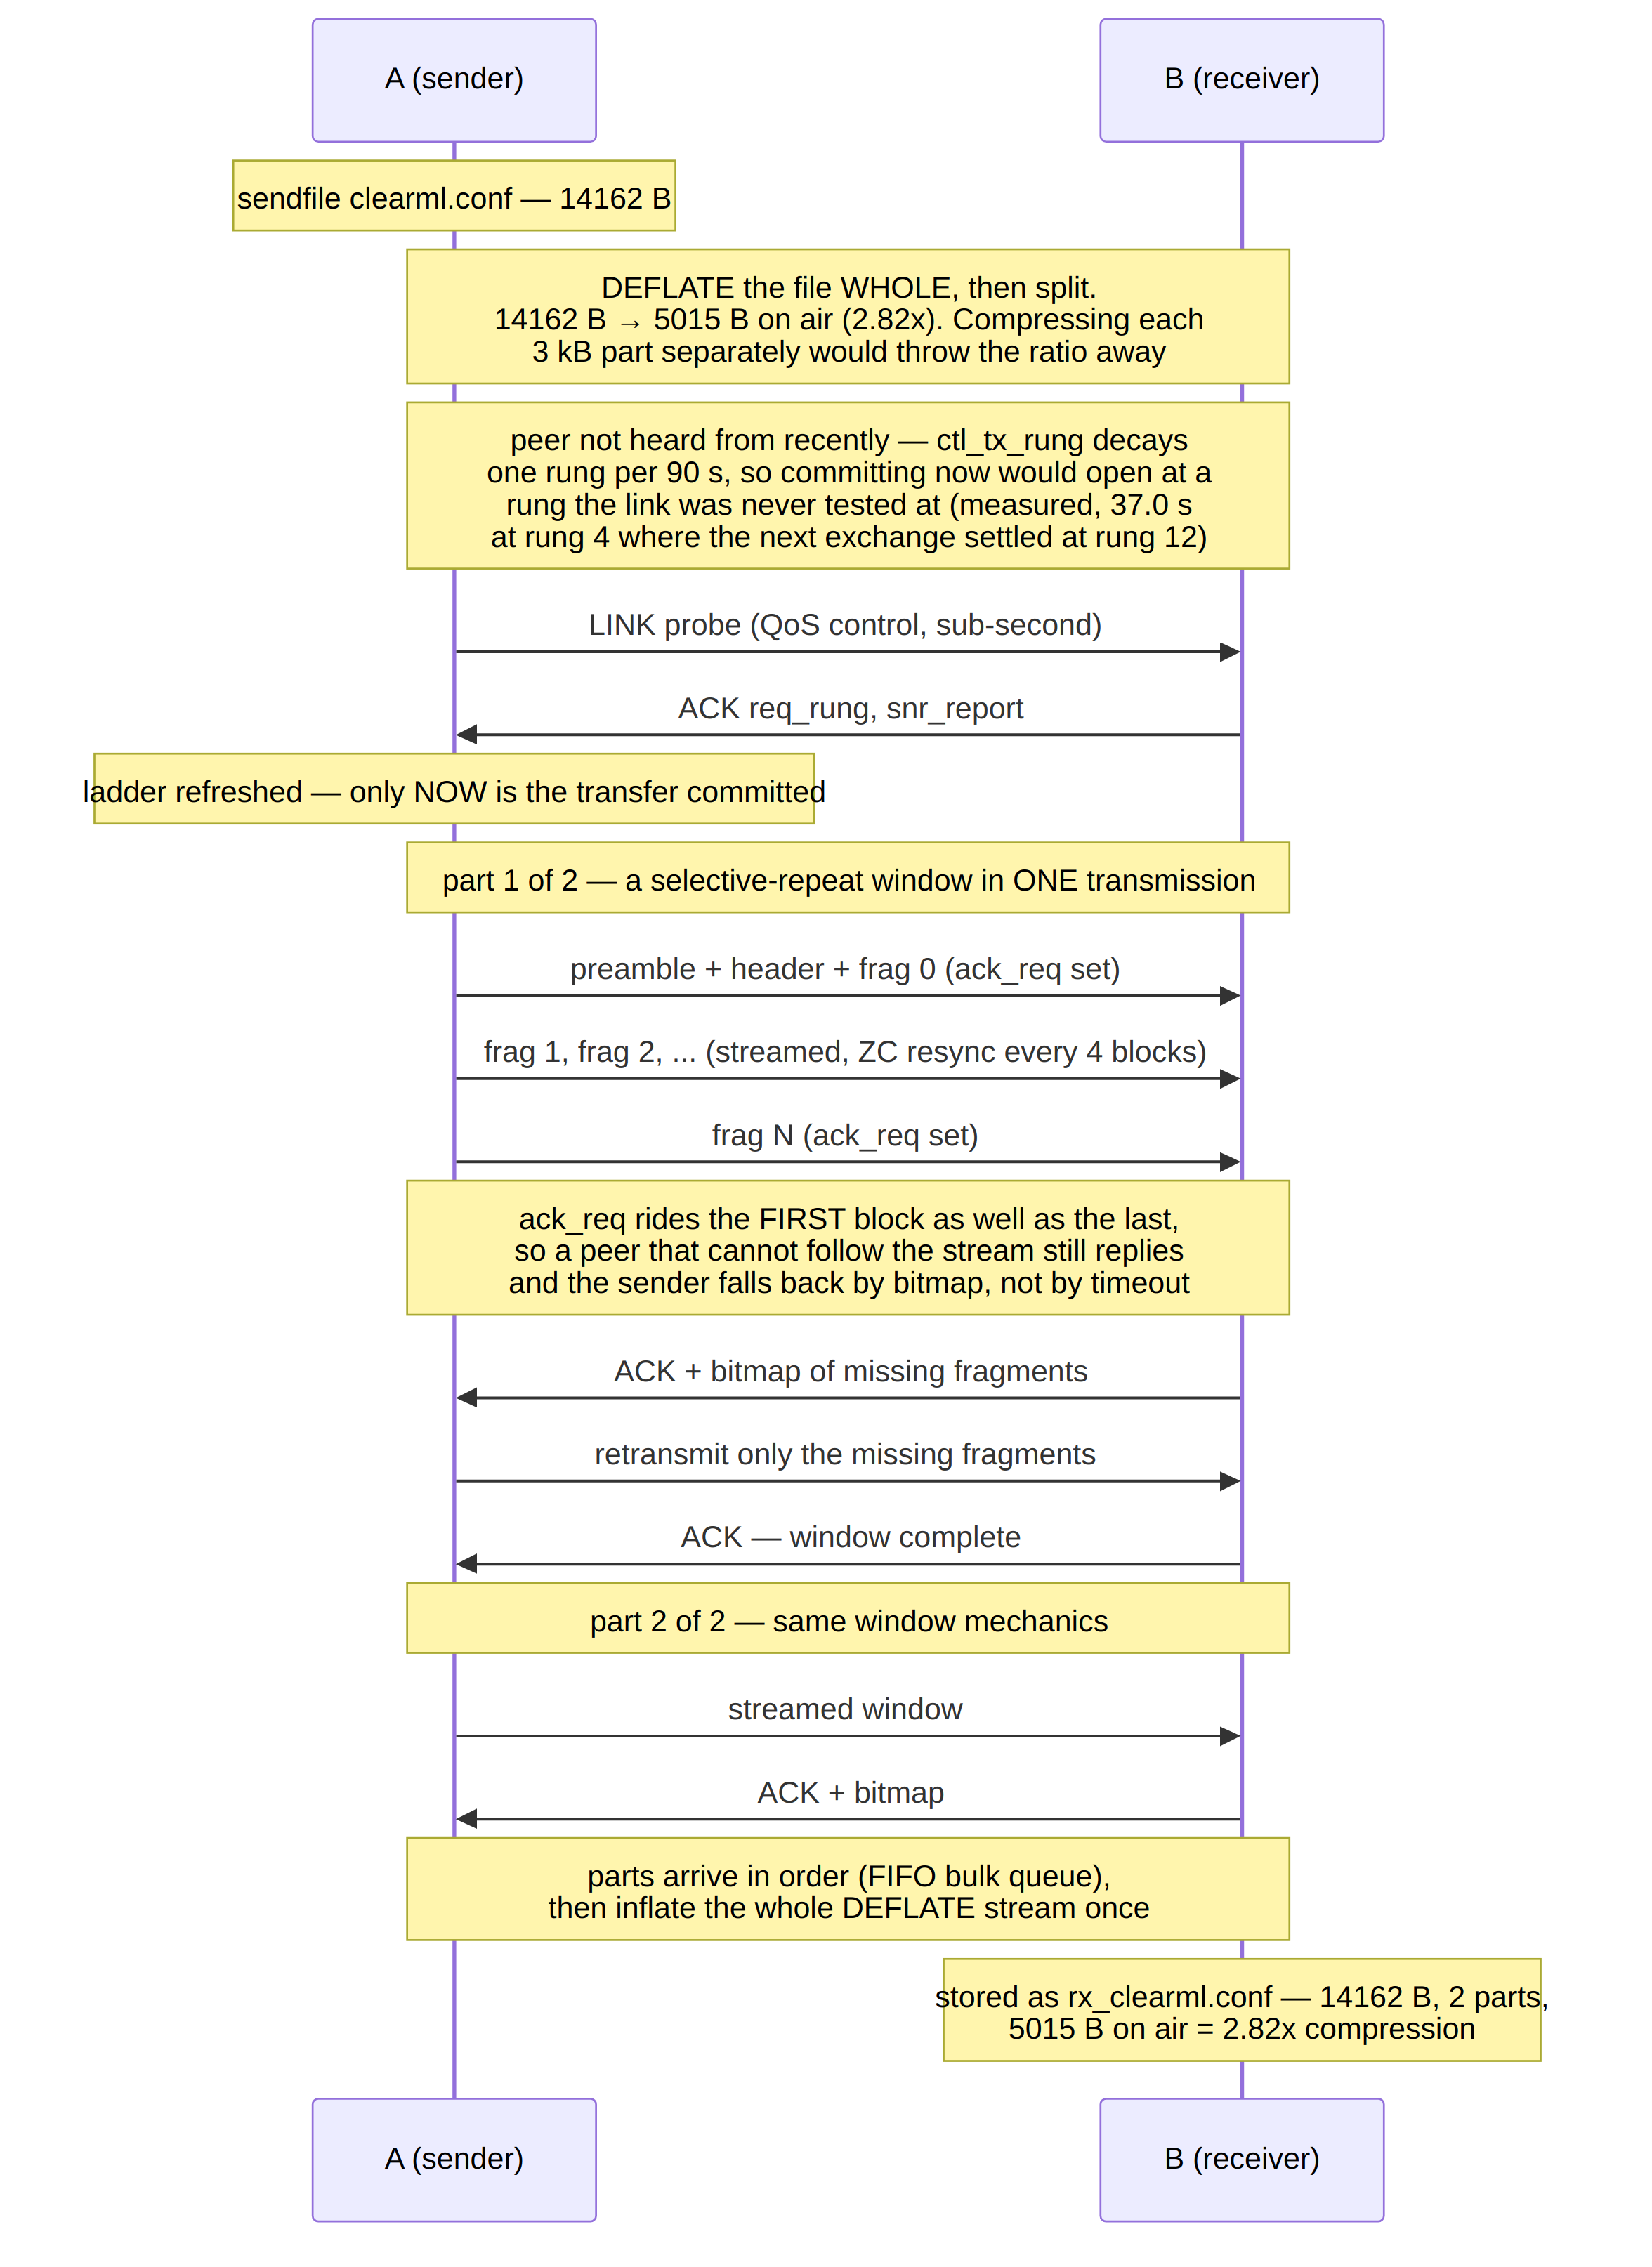
\includegraphics[width=0.90\textwidth]{images/sendfile_seq.png}
    \caption{A file transfer: whole-file compression, a link probe
             before the transfer is committed, then selective-repeat
             windows carried one per transmission.}
    \label{fig:sendfileseq}
\end{figure}

\subsection{From Simulation to a Radio}
\label{sec:cport_sdr}

The demonstration apps talk to a \emph{driver} over a socket rather than
to hardware, which turns out to be the right seam for real radio: an SDR
driver (\texttt{demoapp/sdr\_driver.py}) presenting the same devices puts
the entire C stack on the air with nothing in \texttt{cport/} changed.
It reproduces the SSB model of Section~\ref{sec:rf} sample by sample ---
audio $\rightarrow$ analytic signal (the receiver's own 63-tap Hilbert
design) $\rightarrow$ interpolation to the SDR rate $\rightarrow$ I/Q,
and back, where taking the real part of the decimated baseband
\emph{is} a product detector.  Tuning the radio to the suppressed
carrier makes the two stations' LO error appear as exactly the
audio-band CFO the modem already tracks.  The DSP costs 4.4\,\% of one
core to transmit and 3.1\,\% to receive per audio-second at 2.4\,Msps,
so a laptop runs it comfortably in real time.

Figure~\ref{fig:sdr_setup_loopback} shows the arrangement that needs no
radio at all: the driver cross-connects two stations through the entire
SSB chain --- Hilbert transform, interpolation, int8 quantisation,
decimation and product detection --- so every line of the signal path is
exercised, and the console apps above it cannot tell the difference.
That is what the regression test uses.

\begin{figure}[H]
    \centering
    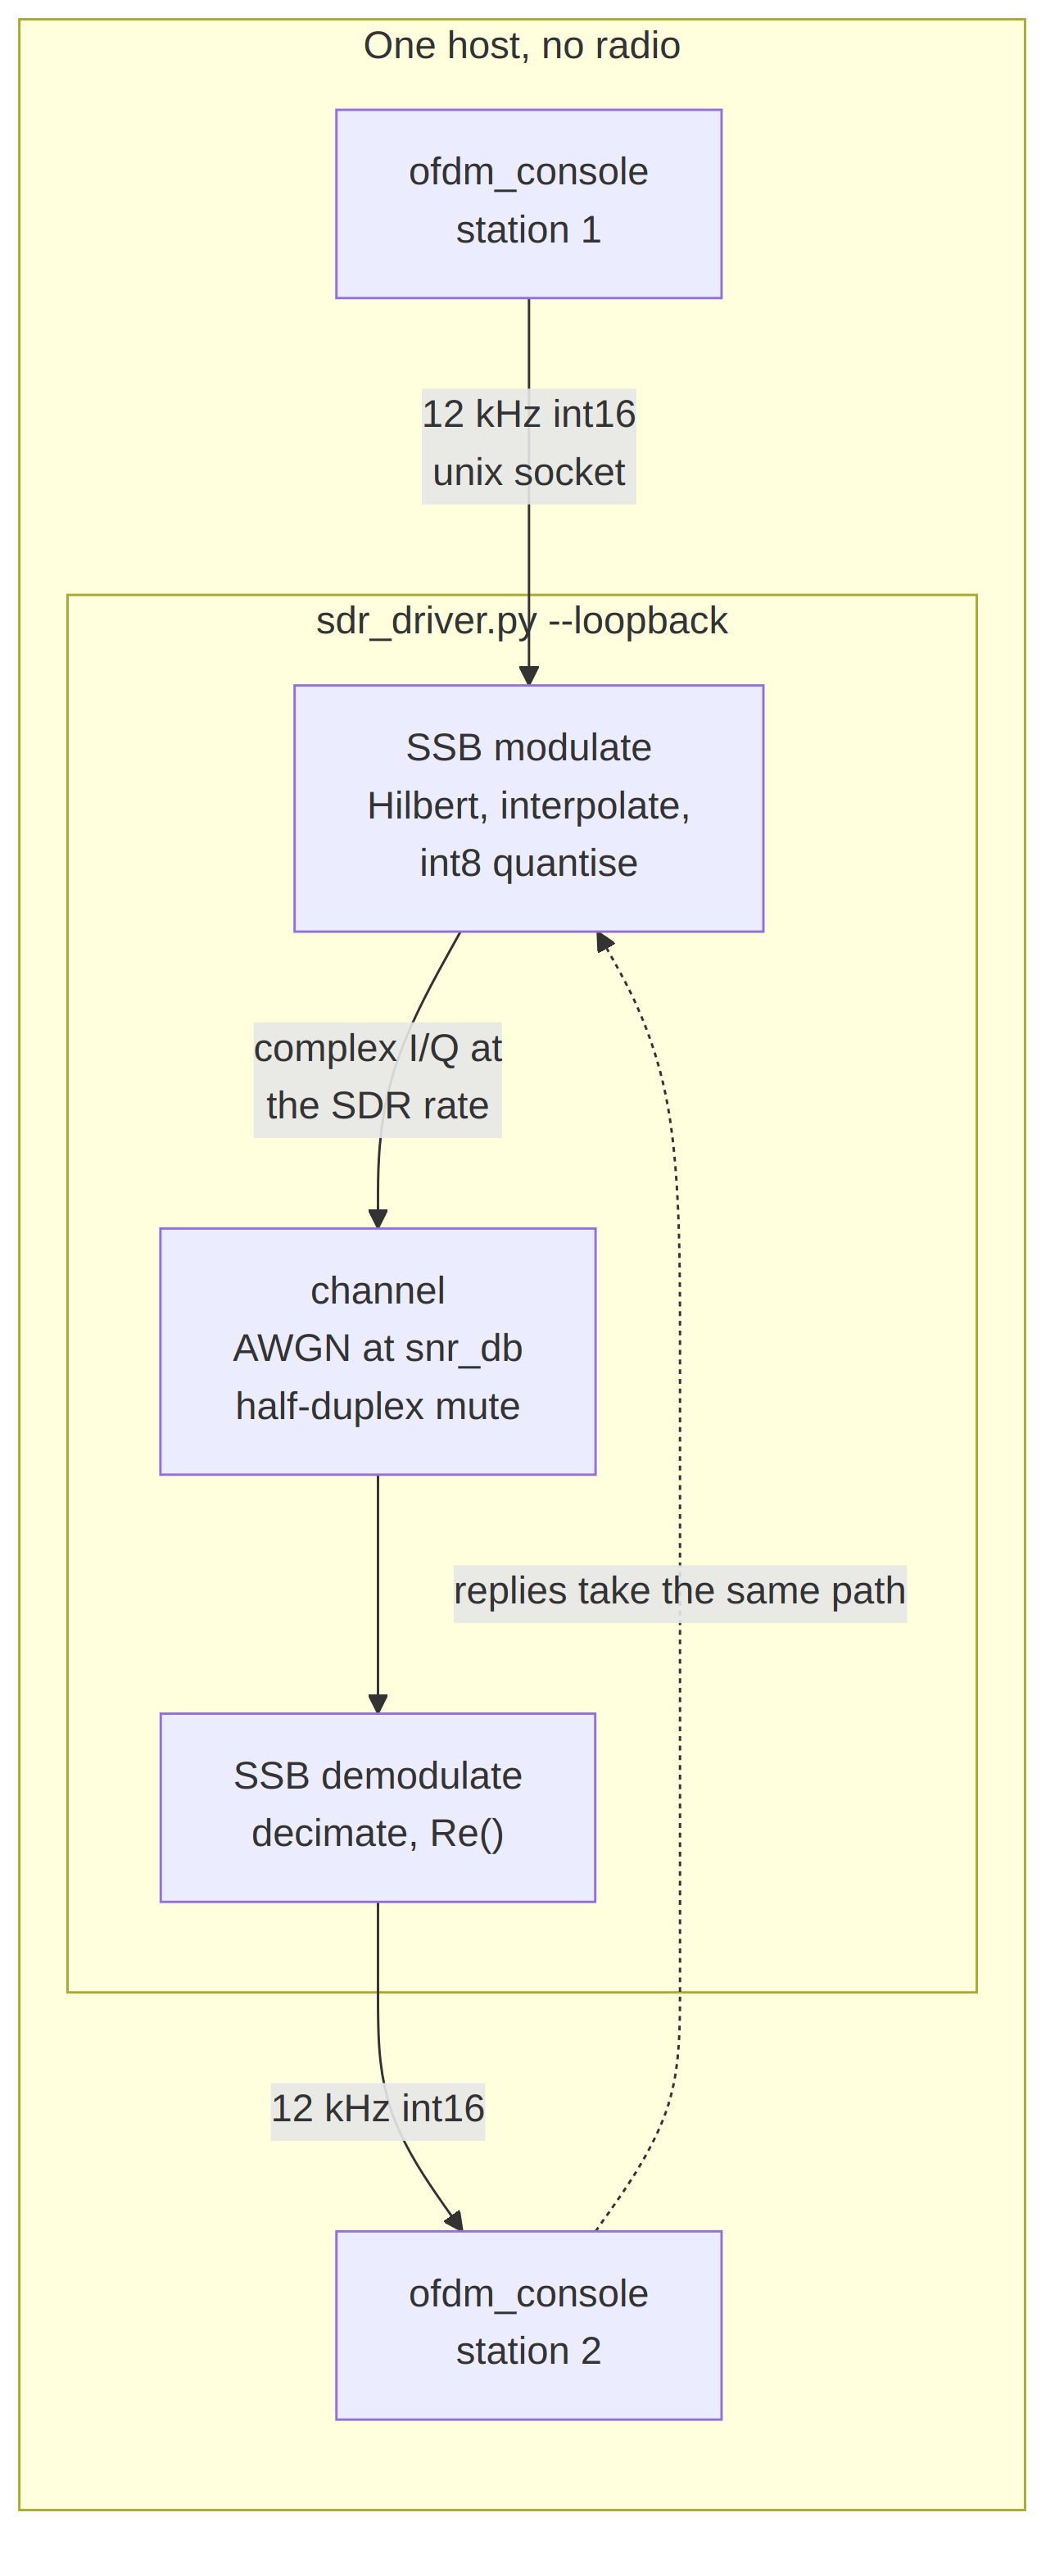
\includegraphics[width=\textwidth]{images/sdr_setup_loopback.png}
    \caption{Hardware-free loopback: two stations cross-connected
             through the full SSB modulation and demodulation chain.}
    \label{fig:sdr_setup_loopback}
\end{figure}

Bringing this up on a HackRF One produced four corrections that no
amount of loopback testing would have found: the local oscillator must
be \emph{offset tuned} (with it on the carrier, the DC leakage lands
inside the 3.5\,kHz passband and the recovered audio was 98\,\% DC ---
the device has neither hardware DC correction nor AGC); the aggregate
gain control is inert and the LNA/VGA/AMP stages must be driven
individually (worth 32\,dB of working level); \texttt{writeStream} only
\emph{queues} samples, so switching back to receive when it returns
truncated the tail of every frame; and a killed process left the radio
\emph{keyed} until a receive stream was opened.

\subsubsection{Instrumented Measurements}

The two measurements that follow share the arrangement of
Figure~\ref{fig:sdr_setup_analyzer}: a tinySA Ultra on USB, used in
both directions.  As an analyser it measures what the radio transmits;
as a source --- through its calibration output, which is a reference
tone at a documented level --- it measures what the receiver makes of a
known input.  Both are scripted, so the numbers below are reproducible
rather than read off a screen.

\begin{figure}[H]
    \centering
    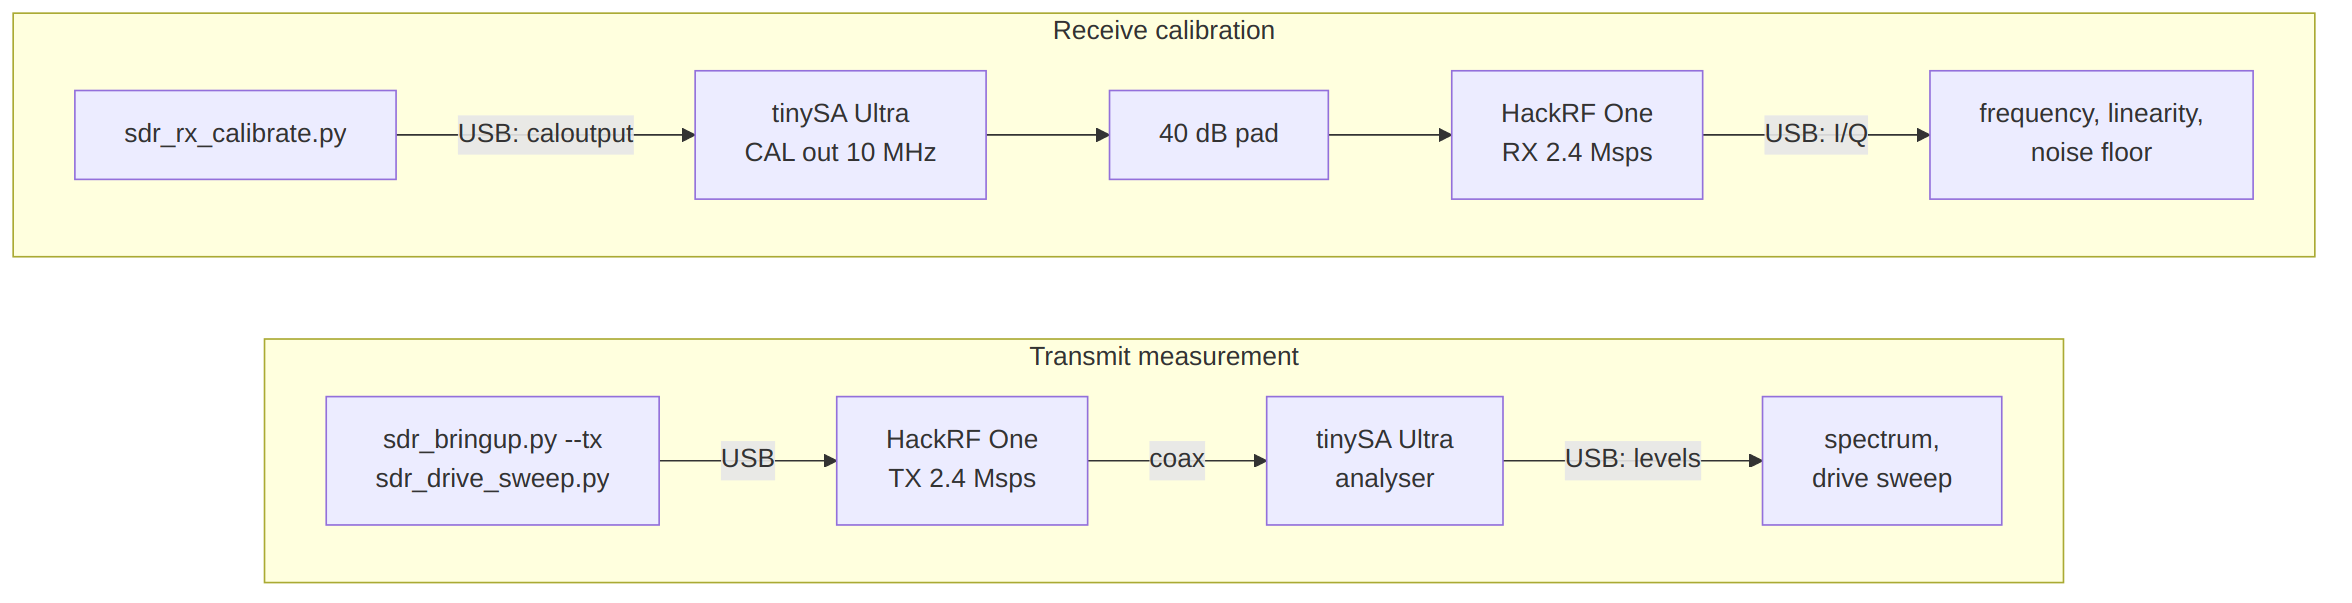
\includegraphics[width=\textwidth]{images/sdr_setup_analyzer.png}
    \caption{Instrumented bench, both directions: as an analyser the
             tinySA measures what the radio transmits; as a source its
             calibration output drives the receiver through a 40\,dB
             pad.}
    \label{fig:sdr_setup_analyzer}
\end{figure}

\subsubsection{The Transmitted Spectrum}

Figure~\ref{fig:sdr_tx_spectrum} is the waveform measured on a tinySA
Ultra wired to the antenna port, captured by
\texttt{demoapp/tinysa.py} (which sweeps with the transmitter off,
keys it, and max-holds several sweeps).  The occupied band matches the
design: a $-3$\,dB width of 2.42\,kHz against the 2.1\,kHz the
numerology predicts, once the 3\,kHz resolution bandwidth is allowed
for, sitting exactly where the carrier and 300--2400\,Hz audio band put
it.  That single measurement validates the absolute tuning, the
offset-tuning arithmetic, the drive scaling into the 8-bit DAC and the
single-sideband modulation at once --- an error in any of them shows up
as splatter or a mirror image.  Visible 50\,kHz below the signal is the
LO leakage at $-35$\,dBc, the price of the offset tuning that keeps DC
out of the \emph{receive} passband.

\begin{figure}[H]
    \centering
    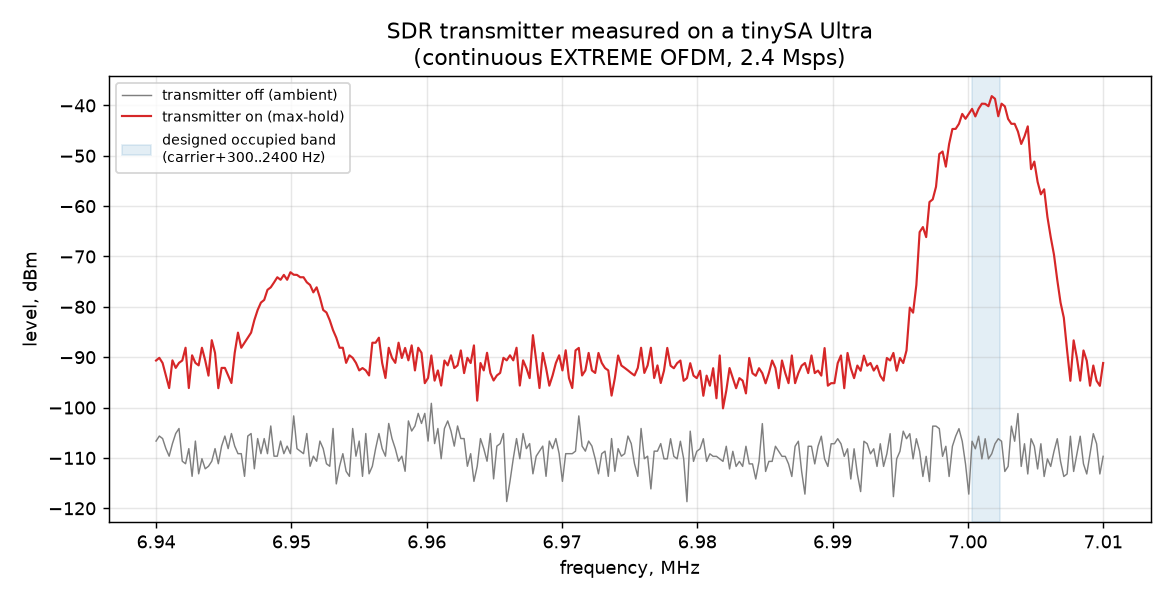
\includegraphics[width=0.92\textwidth]{images/sdr_tx_spectrum.png}
    \caption{The transmitter measured on a tinySA Ultra: continuous
             EXTREME OFDM at 2.4\,Msps, carrier 7.000\,MHz, 3\,kHz RBW.
             The shaded band is the designed occupancy
             (carrier\,$+$\,300\ldots2400\,Hz); the spur at 6.95\,MHz is
             the offset-tuned local oscillator.}
    \label{fig:sdr_tx_spectrum}
\end{figure}

\subsubsection{How Hard the Radio Can Be Driven}

Figure~\ref{fig:sdr_drive_sweep} sweeps the transmit gain and measures,
at each step, the fundamental, the shoulders 5--10\,kHz outside the
occupied band, and the harmonics.  It should be read from the middle
outwards: below VGA 16 the reported shoulders are the \emph{analyser's}
noise floor rather than the transmitter's, because the fundamental is
only $-58$\,dBm.  Above VGA 32 the degradation is real compression,
provoked by the waveform's $\approx$8\,dB PAPR --- at full drive the
shoulders reach $-22$\,dBc and the second harmonic $-38$\,dBc, both
worse than the $-43$\,dBc usually demanded of spurious emissions.

The asymmetry between the two impairments is the practical result: a
low-pass filter removes the harmonics but does nothing about the
shoulders, which are spectral regrowth a few kilohertz from the carrier
and inside any filter's passband.  The usable window with this waveform
is therefore about VGA 16--32, i.e.\ $-42$ to $-24$\,dBm, and real power
has to come from a \emph{linear} external amplifier rather than from
winding this one up --- the same linearity requirement the OFDM
waveform imposes everywhere else in the chain.

\begin{figure}[H]
    \centering
    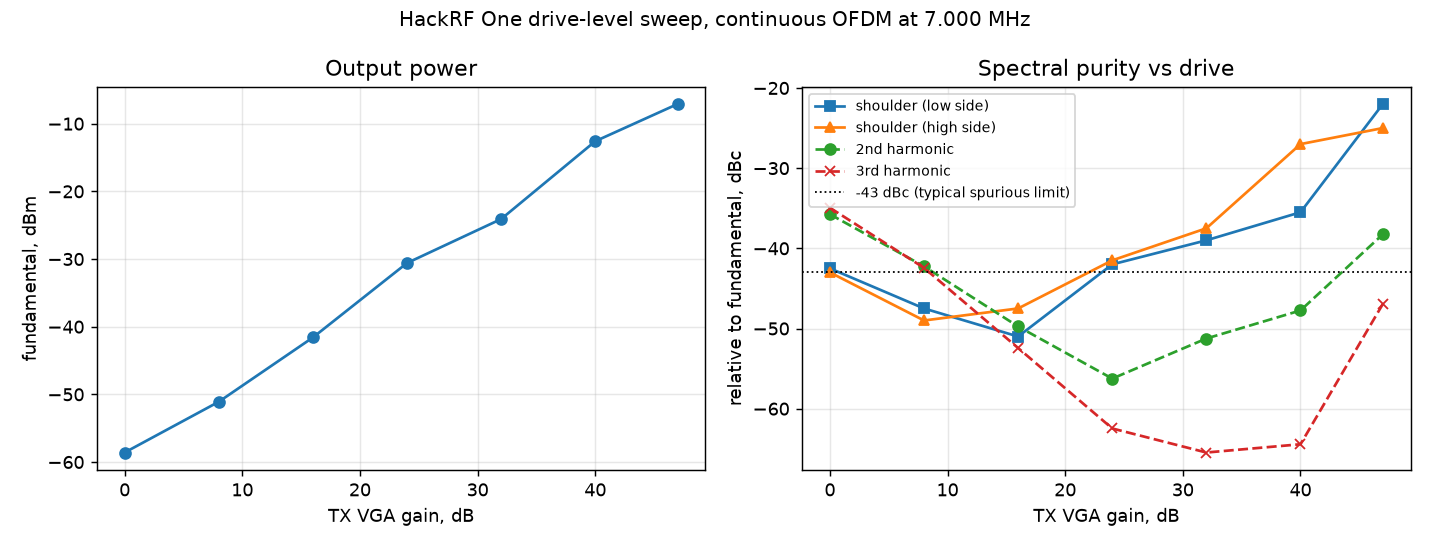
\includegraphics[width=\textwidth]{images/sdr_drive_sweep.png}
    \caption{Drive-level sweep on the HackRF One
             (\texttt{demoapp/sdr\_drive\_sweep.py}): output power, and
             spectral purity relative to the fundamental, against
             transmit gain.  Points below VGA 16 are limited by the
             analyser's noise floor, not by the transmitter.}
    \label{fig:sdr_drive_sweep}
\end{figure}

\subsubsection{Decoding Off the Air}

A half-duplex radio cannot receive its own transmission, so the last
question --- does a receiver actually \emph{decode} this over a real RF
path? --- needs a separate transmitter.  Figure~\ref{fig:sdr_setup_ammod}
shows the one used: a laptop's sound card plays a generated file into an
AM modulator carried by an external generator at 7.000\,MHz, and the
result reaches the SDR through a 40\,dB pad.

AM demands a different detector, for a reason worth stating because it
is a property of the waveform rather than an inconvenience.  The
receiver is single-sideband: it tunes to a \emph{suppressed} carrier and
takes the real part of the baseband.  Present it with a double-sideband
signal and the lower sideband folds onto the upper one; worse, any
frequency error between the generator and the SDR multiplies the audio
by a slow cosine, splitting every subcarrier in two.  The test therefore
recovers the carrier that AM conveniently provides, derotates by it so
the carrier sits at exactly 0\,Hz and zero phase, and only then takes
the real part.  That is classical synchronous detection, and it is why
the decoded CFO in Table~\ref{tab:offair} reads zero: the carrier lock
has already absorbed the error the modem would otherwise estimate.

\begin{figure}[H]
    \centering
    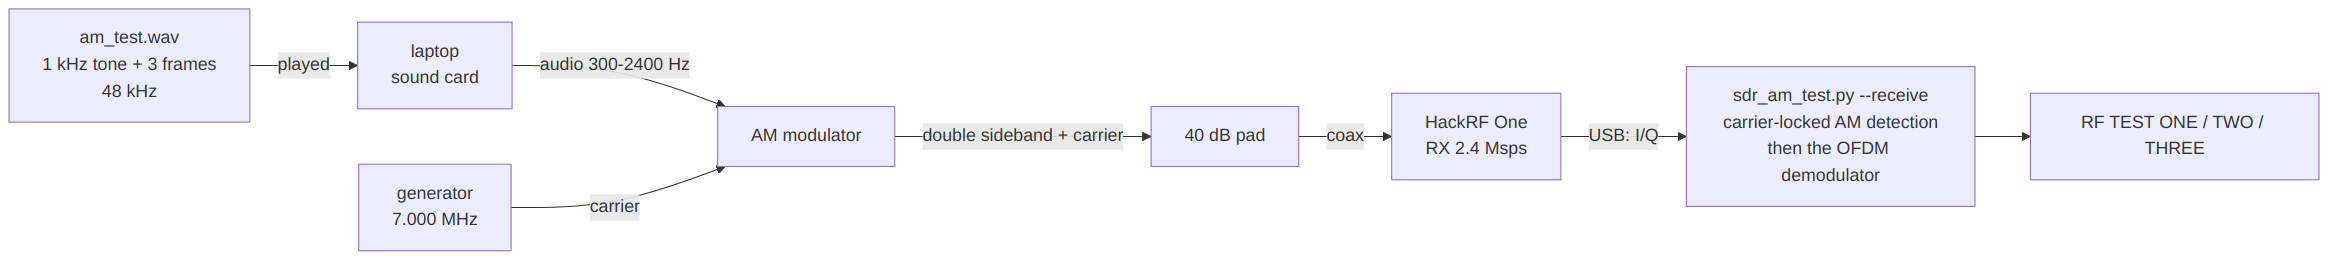
\includegraphics[width=\textwidth]{images/sdr_setup_ammod.png}
    \caption{Off-air receive test: an external AM transmitter feeds the
             SDR through a 40\,dB pad.}
    \label{fig:sdr_setup_ammod}
\end{figure}

\begin{table}[H]
    \centering
    \caption{All three transmitted frames recovered over a 7\,MHz RF
             path (\texttt{results/am\_rx\_offair.wav}).}
    \label{tab:offair}
    \small
    \begin{tabular}{@{}llrr@{}}
    \toprule
    \textbf{Frame} & \textbf{Payload} & \textbf{Length} &
    \textbf{SNR} \\
    \midrule
    NORMAL QPSK 1/2 & \texttt{RF TEST ONE}   & 1.0\,s & $+13.6$\,dB \\
    NORMAL BPSK 1/3 & \texttt{RF TEST TWO}   & 1.8\,s & $+14.4$\,dB \\
    ROBUST BPSK 1/3 & \texttt{RF TEST THREE} & 7.3\,s & $+8.5$\,dB \\
    \bottomrule
    \end{tabular}
\end{table}

Figure~\ref{fig:sdr_waterfall} is what those frames look like as the
demodulator received them.  The analysis FFT is 128 bins at 12\,kHz,
which is exactly the modem's own subcarrier grid, so every row of the
waterfall is one OFDM bin and the structure of
Section~\ref{sec:phy} is directly legible: the Newman tone comb
striping the preamble, then the header, then the data block filling
300--2400\,Hz.  The two NORMAL frames last about a second; the ROBUST
frame occupies 7.35\,s for the same 27 bytes, which is what
$16\times$ tiling costs and buys.  The region boundaries are not
fitted --- they are computed from the decoded header's own modulation,
code rate and length fields, and land on the measured burst to within
15\,ms.

\begin{figure}[H]
    \centering
    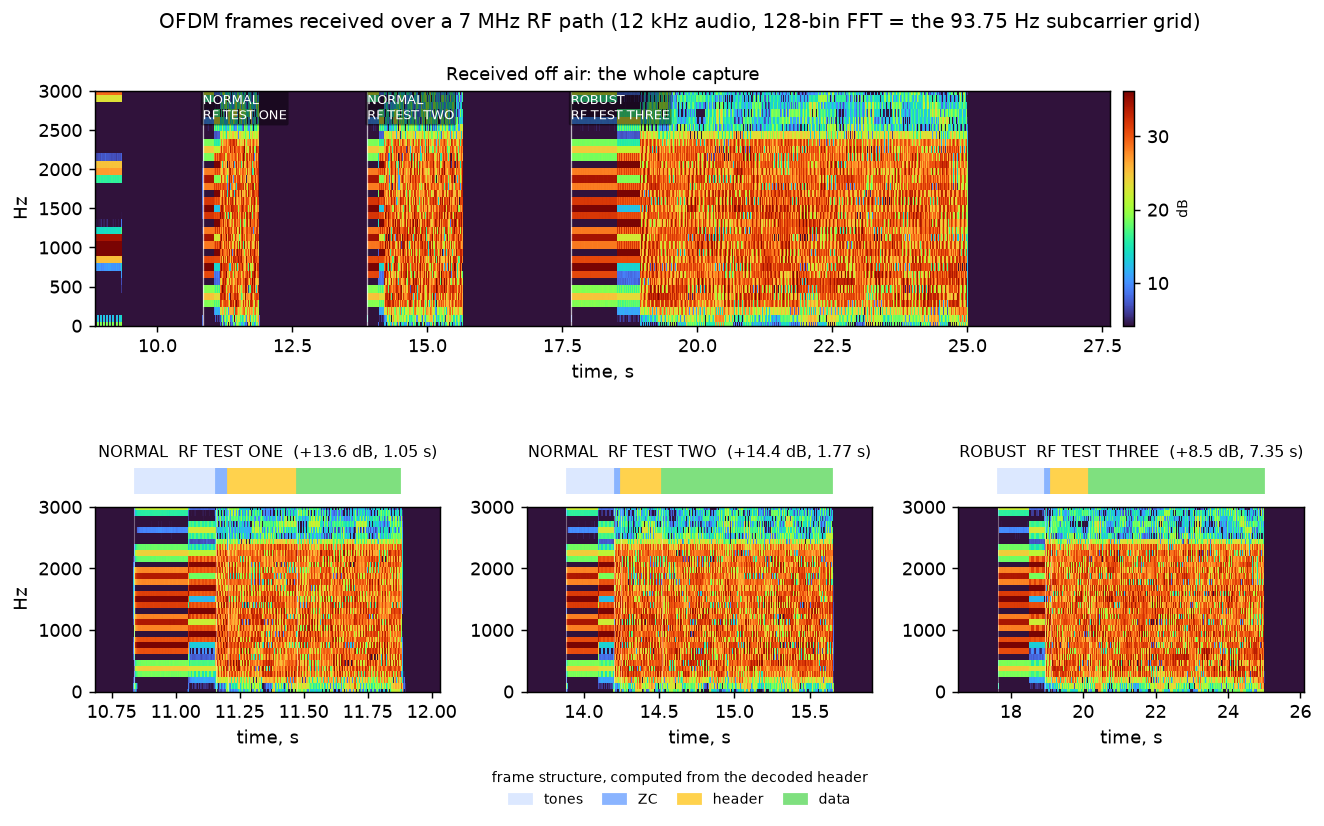
\includegraphics[width=\textwidth]{images/sdr_waterfall.png}
    \caption{Frames received over the air (\texttt{demoapp/sdr\_waterfall.py}
             on \texttt{results/am\_rx\_offair.wav}): the whole capture
             above, each frame close up below with its preamble, header
             and data spans marked.}
    \label{fig:sdr_waterfall}
\end{figure}

Figure~\ref{fig:sdr_waterfall} shows those frames as the demodulator
received them.  The analysis FFT is 128 bins at 12\,kHz, exactly the
modem's own subcarrier grid, so each row is one OFDM bin and the frame
structure of Section~\ref{sec:phy} is directly legible: the Newman tone
comb lighting only a few bins, the Zadoff--Chu symbol closing the
preamble, then the header and the data block filling 300--2400\,Hz.
The spans above each waterfall are computed rather than fitted --- from
the mode's tone-field geometry and the decoded header's own modulation,
code rate and length --- and they land on the measured burst to within
15\,ms.  The comb's end is measurable independently: bin occupancy sits
at 0.17 through the tone fields and jumps to 0.9 at 0.321\,s, against a
predicted 0.320\,s.  It is worth noting that the ZC symbol occupies all
23 carriers, so on a waterfall it resembles data even though it belongs
to the preamble --- which is why it is drawn as its own span.

\begin{figure}[H]
    \centering
    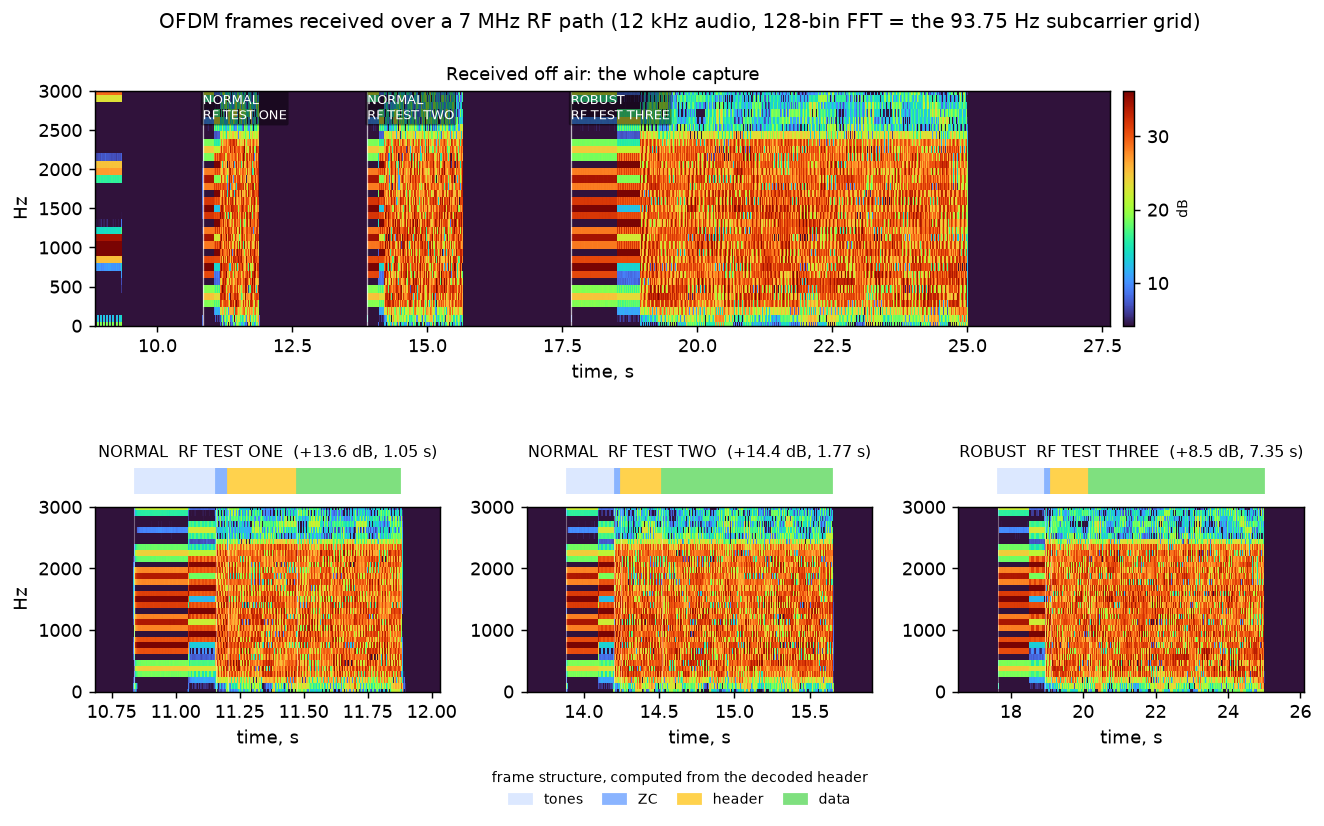
\includegraphics[width=\textwidth]{images/sdr_waterfall.png}
    \caption{Frames received over the air
             (\texttt{demoapp/sdr\_waterfall.py} on
             \texttt{results/am\_rx\_offair.wav}): the whole capture
             above, each frame below with its measured structure.  The
             ROBUST frame carries the same 27 bytes as its NORMAL
             neighbours and occupies 7.35\,s doing it --- what
             $16\times$ tiling costs, and buys.}
    \label{fig:sdr_waterfall}
\end{figure}

Every frame transmitted was recovered, across two link modes and two
modulations, with the mode identified from the preamble root alone ---
the mechanism the whole adaptive ladder depends on, here exercised over
real RF rather than in simulation.  ROBUST reports the lowest SNR by
design: its $16\times$ tiling spreads the same energy over a longer
symbol, so the per-symbol estimate falls while the decoded margin grows.

Two honest qualifications.  The transmitter is an AM modulator rather
than the SDR of the preceding sections, so this validates the receive
chain over RF and not a complete transmit-to-receive loop, which still
wants a second radio.  And a first, coarser scan of the same recording
found only two of the three frames, because it advanced four seconds
after each hit while the demodulator returns one frame per window ---
the miss was in the measurement harness, not the link, which is exactly
the kind of result worth re-checking before blaming the hardware.
